\documentclass[12pt,]{article}
\usepackage{lmodern}
\usepackage{amssymb,amsmath}
\usepackage{ifxetex,ifluatex}
\usepackage{fixltx2e} % provides \textsubscript
\ifnum 0\ifxetex 1\fi\ifluatex 1\fi=0 % if pdftex
  \usepackage[T1]{fontenc}
  \usepackage[utf8]{inputenc}
\else % if luatex or xelatex
  \ifxetex
    \usepackage{mathspec}
  \else
    \usepackage{fontspec}
  \fi
  \defaultfontfeatures{Ligatures=TeX,Scale=MatchLowercase}
\fi
% use upquote if available, for straight quotes in verbatim environments
\IfFileExists{upquote.sty}{\usepackage{upquote}}{}
% use microtype if available
\IfFileExists{microtype.sty}{%
\usepackage{microtype}
\UseMicrotypeSet[protrusion]{basicmath} % disable protrusion for tt fonts
}{}
\usepackage[margin=1.5in]{geometry}
\usepackage{hyperref}
\hypersetup{unicode=true,
            pdftitle={A climate selection experiment with 517 Arabidopsis thaliana ecotypes},
            pdfauthor={Moises Exposito-Alonso1 , Rocío Gómez Rodríguez2, Cristina Barragán1, Giovanna Capovilla1, Eunyoung Chae1, Jane Devos1, Ezgi Dogan1, Claudia Friedemann1, Caspar Gross1, Patricia Lang1, Derek Lundberg1, Belén Méndez-Vigo3, Vera Middendorf1, Jorge Kageyama1, Talia Karasov1, Sonja Kersten1, Sebastian Petersen1, Leily Rabbani1, Julian Regalado1, Beth Rowan1, Danelle Seymour1, Efthymia Symeonidi1, Rebecca Schwab1, Diep Tran1, Kavita Venkataramani1, Anna-Lena Van de Weyer1, George Wang1, Ronja Wedegärtner1, Frank Weiss1, Rui Wu1, Wanyan Xi1, Maricris Zaidem1, Wangsheng Zhu1, Fernando García Arenal2, Carlos Alonso Blanco3, Xavier Picó4, Hernán A. Burbano1, Oliver Bossdorf5, Detlef Weigel1.  Max Planck Institute for Developmental Biology, Tübingen, Germany  Centre for Plant Biotechnology and Genomics, Technical University of Madrid, Pozuelo de Alarcón, Spain  National Centre of Biotechnology, Cantoblanco, Madrid, Spain  Doñana Biological Station, Sevilla, Spain  University of Tübingen, Tübingen, Germany},
            pdfkeywords={Arabidopsis thaliana, natural selection, field experiments, climate
change},
            pdfborder={0 0 0},
            breaklinks=true}
\urlstyle{same}  % don't use monospace font for urls
\usepackage{graphicx,grffile}
\makeatletter
\def\maxwidth{\ifdim\Gin@nat@width>\linewidth\linewidth\else\Gin@nat@width\fi}
\def\maxheight{\ifdim\Gin@nat@height>\textheight\textheight\else\Gin@nat@height\fi}
\makeatother
% Scale images if necessary, so that they will not overflow the page
% margins by default, and it is still possible to overwrite the defaults
% using explicit options in \includegraphics[width, height, ...]{}
\setkeys{Gin}{width=\maxwidth,height=\maxheight,keepaspectratio}
\IfFileExists{parskip.sty}{%
\usepackage{parskip}
}{% else
\setlength{\parindent}{0pt}
\setlength{\parskip}{6pt plus 2pt minus 1pt}
}
\setlength{\emergencystretch}{3em}  % prevent overfull lines
\providecommand{\tightlist}{%
  \setlength{\itemsep}{0pt}\setlength{\parskip}{0pt}}
\setcounter{secnumdepth}{0}
% Redefines (sub)paragraphs to behave more like sections
\ifx\paragraph\undefined\else
\let\oldparagraph\paragraph
\renewcommand{\paragraph}[1]{\oldparagraph{#1}\mbox{}}
\fi
\ifx\subparagraph\undefined\else
\let\oldsubparagraph\subparagraph
\renewcommand{\subparagraph}[1]{\oldsubparagraph{#1}\mbox{}}
\fi

%%% Use protect on footnotes to avoid problems with footnotes in titles
\let\rmarkdownfootnote\footnote%
\def\footnote{\protect\rmarkdownfootnote}

%%% Change title format to be more compact
\usepackage{titling}

% Create subtitle command for use in maketitle
\newcommand{\subtitle}[1]{
  \posttitle{
    \begin{center}\large#1\end{center}
    }
}

\setlength{\droptitle}{-2em}
  \title{A climate selection experiment with 517 \emph{Arabidopsis thaliana}
ecotypes}
  \pretitle{\vspace{\droptitle}\centering\huge}
  \posttitle{\par}
  \author{\newline \normalfont Moises
Exposito-Alonso\textsuperscript{1}\textsuperscript{*} , Rocío Gómez
Rodríguez\textsuperscript{2}, Cristina Barragán\textsuperscript{1},
Giovanna Capovilla\textsuperscript{1}, Eunyoung Chae\textsuperscript{1},
Jane Devos\textsuperscript{1}, Ezgi Dogan\textsuperscript{1}, Claudia
Friedemann\textsuperscript{1}, Caspar Gross\textsuperscript{1}, Patricia
Lang\textsuperscript{1}, Derek Lundberg\textsuperscript{1}, Belén
Méndez-Vigo\textsuperscript{3}, Vera Middendorf\textsuperscript{1},
Jorge Kageyama\textsuperscript{1}, Talia Karasov\textsuperscript{1},
Sonja Kersten\textsuperscript{1}, Sebastian Petersen\textsuperscript{1},
Leily Rabbani\textsuperscript{1}, Julian Regalado\textsuperscript{1},
Beth Rowan\textsuperscript{1}, Danelle Seymour\textsuperscript{1},
Efthymia Symeonidi\textsuperscript{1}, Rebecca
Schwab\textsuperscript{1}, Diep Tran\textsuperscript{1}, Kavita
Venkataramani\textsuperscript{1}, Anna-Lena Van de
Weyer\textsuperscript{1}, George Wang\textsuperscript{1}, Ronja
Wedegärtner\textsuperscript{1}, Frank Weiss\textsuperscript{1}, Rui
Wu\textsuperscript{1}, Wanyan Xi\textsuperscript{1}, Maricris
Zaidem\textsuperscript{1}, Wangsheng Zhu\textsuperscript{1}, Fernando
García Arenal\textsuperscript{2}, Carlos Alonso
Blanco\textsuperscript{3}, Xavier Picó\textsuperscript{4}, Hernán A.
Burbano\textsuperscript{1}, Oliver Bossdorf\textsuperscript{5}, Detlef
Weigel\textsuperscript{1}. \newline \small \newline \textsuperscript{1}
Max Planck Institute for Developmental Biology, Tübingen, Germany
\newline \textsuperscript{2} Centre for Plant Biotechnology and
Genomics, Technical University of Madrid, Pozuelo de Alarcón, Spain
\newline \textsuperscript{3} National Centre of Biotechnology,
Cantoblanco, Madrid, Spain \newline \textsuperscript{4} Doñana
Biological Station, Sevilla, Spain \newline \textsuperscript{5}
University of Tübingen, Tübingen, Germany \newline 
\newline \newline \newline \newline \newline \newline}
  \preauthor{\centering\large\emph}
  \postauthor{\par}
  \date{}
  \predate{}\postdate{}

\usepackage{hyperref}
\usepackage{caption}
\usepackage{subcaption}
\usepackage{graphicx}
\usepackage[nomarkers,figuresonly]{endfloat}

\begin{document}
\maketitle
\begin{abstract}
To quantify phenotypic and genetic natural selection, the gold standard
are evolution experiments. However, studies that include whole-genome
data are still scarce. Evolution experiments can be longitudinal, as
laboratory experiments continued over many generations, or
cross-sectional, as field experiments replicated over many geographic
locations or environments. For long-lived organisms (generation time
over a 1 year) such as \textit{Arabidopsis thaliana}, only
cross-sectional studies are most feasible. Here we present an experiment
carried out in a Mediterranean and a Central European field station and
in which we additionally manipulated rainfall. We used 517 whole-genome
sequenced \textit{A. thaliana} lines covering the global distribution.
We encapsulate the raw data and processing code in an R package
``dryAR'' available at
\url{http://github.com/MoisesExpositoAlonso/updatehere}. We believe this
could be a useful resource for the evolutionary biology and the
Arabidopsis communities.
\end{abstract}

\section{Field experiment design}\label{field-experiment-design}

\subsection{The ecotypes from the 1001 Genomes
Projects}\label{the-ecotypes-from-the-1001-genomes-projects}

The 1001 project (1001 Genomes Consortium 2016) comprises 1135 accession
lines (or ecotypes) sequenced (Fig. \ref{fig:ecotypes}). Here are the
details of the protocol used to select the most informative, less biased
sample of the lines within the 1001 genomes project in order to
prioritize phenotypic efforts. Filtering consisted in several
approaches: (1) First we aimed to remove those accessions with the
lowest genome quality. Among 1135, we discarded those with \textless{}
10X genome coverage and \textless{} 90\% congruence of SNPs called from
Max Planck Institute and Gregor Mendel Institute pipelines (1001 Genomes
Consortium 2016). The remaining number were 959 accessions. (2)
Parallely, we filtered almost-identical individuals. Using Plink we
computed identity by state genome-wide across the 1135 accessions. For
those pairs of accessions with \textless{} 0.01 differences per SNP, we
randomly picked one. This resulted in 889 accessions. The merge between
(1) and (2) criteria was 762. (3) Finally, we reduced geographic
ascertainment. Sampling for the 1001g project was not performed in
either a random nor regular structured scheme. Some laboratories
provided several lines per locations whereas others provided lines that
were at least several hundred kilometres apart. Employing latitude and
longitude degrees, we computed euclidean distances across the 1135
accessions and identified pairs that were \textless{} 0.0001 distance,
that is accessions from the same population ( \textless{}\textless{} 100
meters), and randomly picked one. This resulted in 682 accessions. We
merged the resulting lists of accessions after the three quality
filtering procedures and obtained a final set of 523 accessions. We
reproduced accessions in controlled conditions to generate enough seeds
for the field experiment. A total of 517 accessions were finally planted
in the field experiments (Fig. \ref{fig:ecotypes}).

\subsection{Field settings and
watering}\label{field-settings-and-watering}

We build two 30m x 6m tunnels with similar PVC plastic foils to fully
exclude rainfall in Madrid and in Tübingen (Fig 2). The foil tunnels are
different from a greenhouse in that they are completely opened in two
sides, thus ambient temperatures vary as much as any outdoor experiment
{[}include environmental information{]}. In each location, we supplied
artificial watering at two contrasting regimes: abundant watering and
reduced watering. Inside each tunnel, we created an approximate 10\%
slope and set up four flooding tables in the ground (1m x 25m). The
lower elevation side of the flooding table was used to drain the water
provided from the other, higher elevation, side of the table (Fig 2).
The soil from trays from the two treatments clearly showed a consistent
difference in water content {[}insert environment{]}.

We used trays of 8x5 cells (5.5 x 5.5 x 10cm size). One genotype was
planted per cell. We grew a total of 12 replicates per genotype per
treatment. Five replicates were planted at a density of 30 counted seeds
per cell and were let grow without disturbance (``population
replicate''). Seven were planted at low density (ca. 10 seeds) and once
germinated one seedling was selected at random (``individual
replicate'').

\subsection{Blocking and
randomization}\label{blocking-and-randomization}

We used an incomplete block randomized designed (Fig. \ref{fig:blocks}).
A total of 16 blocks were established. For each watering treatment there
were two blocks, which were intercalated. Within each flooding table
there were four blocks, two of individual replicates and two of
population replicates; also intercalated. Within each watering x
replicate type x replicate number combination block, genotypes were
randomly distributed in the trays (Fig. \ref{fig:trays}). The randomized
designed was identical in Madrid and Tübingen.

\subsection{Removal of errors during sowing and possible
contaminations}\label{removal-of-errors-during-sowing-and-possible-contaminations}

In a large enterprise such as this field experiment, errors can occur.
However, we tried to control such errors by reducing the ``degrees of
freedom'' of the experimenters. We tried to accomplish this by preparing
and curating all eppendorf with the seeds to be sown in cardboard boxes
with the same cells as in the target trays and arranged them in their
corresponding (randomised) locations. Then, during sowing each
experimenter took a box at random and went to the corresponding tray in
the field previously arranged (Fig. S2). This reduced the possibility of
sowing errors, but when an incorrect sowing was done (wrong positions,
badly sprayed), we recorded those and exclude them from the analyses.

We were aware that contamination of neighboring pots was a risk. For
that reason the first watering days were gentle. Furthermore, we pick a
day with no wind and we throw the seeds from 1-2 cm height from the
soil. During the vegetative grow we identified germination that looked
like neighbour contamination and remove those. Although we lost a number
of plants, the power of the design was the replication, thus we
discarded everything that looked suspicious. During the recording of
flowering time, we used the homogeneity of flowering within a pot as a
sign of contamination. When a plant had a completely different flowering
stage and leaf phenotypes did not coincide with the majority of the pot,
this plant was removed.

\section{Recording of flowering time}\label{recording-of-flowering-time}

We visited the field experiment on average every 1 or 2 days and
recorded manually what pots had flowered. To keep track from previous
visits and avoid errors, we sticked blue pins in the pots were flowering
was recorded. This removed a source of human error. To calculate
flowering time, we counted the number of days from the date of sowing to
to the assigned flowering date. Fig. \ref{fig:flowerraw} shows the raw
flowering time data per pot in the original spatial distribution of pots
as in ref\{fig:blocks\}. Fig. \ref{fig:flowerdistribution} shows the
distribution of flowering time per treatment combination. Note that grey
boxes in Fig. \ref{fig:flowerraw} are pots with plants that did not
survive until flowering. For more visualizations of flowering time see
\url{http://github.com/MoisesExpositoAlonso/field/data-cleaning/updatehere}.

\section{Image production and
analysis}\label{image-production-and-analysis}

\subsection{Vegetative rosettes}\label{vegetative-rosettes}

Top-view images were taken every four to five days (median) with a
Panasonic DMC-TZ61 digital camera and a customized closed black box
(Fig. \ref{fig:trays}) at a distance of 40 cm from the tray. Photos were
taken on average every x days from the sowing date until flowering
plants impede the acquisition -- a total of 20 timepoints. Images for
analyses are available at \url{http://datadryad.org/updatehere} and the
software to process and analyse them is available at
\url{http://github.com/MoisesExpositoAlonso/hippo}. Segmentation was
done similarly as Exposito-Alonso \emph{et al.} (2017). We began by
transforming images from RGB to HSV channels. We applied a hard
segmentation threshold of HSV values as (H = 30-65, S=65-255, V=20-220).
This was followed by several iterations of morphology transformations
based on erosion and dilation. Then, for the resulting binary image we
counted the number of green pixels. During field monitoring we noticed
that some pots did not germinate. Sometimes this was due to lack of
seeds or improper soil compaction. In those cases, we left a red mark in
those pots, which we could detect in the same way as the existence of
green pixels (with threshold H=150-179, S=100-255, V=100-255). Those
pots were excluded from survival analyses as they contained any plants.
An example of transformed images is in Figure \ref{fig:segmentation}.

The resulting raw data consists in green and red area (pixel counts) per
pots (Fig. \ref{fig:pixels}A). We took the advantage that a tray was
photographed the same day several times to verify the replicability of
our pipeline. In total there were 790 of such observations distributed
in 11 timepoint and different trays. Using the R package lme4 1.1-12
(Bates \emph{et al.} (2015)), we computed a generalized linear mixed
model with Poisson distribution (Bolker \emph{et al.} 2009), and derived
the variance proportion of pixel counts explained by the pot identity
taken at the same day: \(Var_{green} / Var_{tot} = 99.7 \%\). As this
replicability proportion was high, we summarized the mean number of
green pixels for those duplicated pots.

In order to remove from the analyses those pots that did not germinate,
we performed a moving threshold and analysis of variance to determine
what is the number of red pixels above which a pot is highly likely to
have a red mark. As expected, the distribution of pixels is bimodal
(Fig. \ref{fig:red}), what makes this process straightforward and
reliable. This filtering lead to a dataset of 434240 pixel observations
(from an original of 474100).

Then we aimed to quantify germination timing. We did this by modeling
the growth trajectory of green pixels per pot as a sigmoidal curve
fitting the next function:

\[y = \frac{a}{1 + e^{-(b  \times   (x-c))} } \] , starting in the
sowing day and until the observed peak of green pixels per pot. The
three parameters \(a\), \(b\), and \(c\), would inform about the
different shapes of growth curves. We also computed less complex
indicators of growth: an analogous linear model that was used to
determine the intersection with 1000 pixels, the day that over 1000
green pixels were observed (\textasciitilde{} 1cm\textsuperscript{2} as
pixels resolution is \textasciitilde{}xyz), the day that a fitted spline
passed over 1000 green pixels, and a total count of green and red pixels
through all timepoints. In Fig. \ref{fig:trajectories}, we show a total
of 1000 example growth trajectories modeled with the sigmoidal approach
and in Fig. \ref{fig:germination} we show the estimated number of days
from sowing till germination based on the spline approach. The final
dataset comprised 22779 observations with germination day from low
complex indicators, and 12636 for which a sigmoidal curve could be
fitted. A detailed R markdown document of data loading and cleaning can
be found at
\url{http://github.com/MoisesExpositoAlonso/field/data-cleaning/updatehere}.

\subsection{Reproductive plants}\label{reproductive-plants}

Once flowering plants finished the reproductive stage (dry fruits were
observed), we harvested them and took a final photograph of the rosette
and the inflorescence (Fig. \ref{fig:skeletonisation}). The python
module to analyse the inflorescence pictures (Fig. \ref{fig:original})
is available at \url{http://github.com/MoisesExpositoAlonso/hitfruit}.
We first used a cycle of morphological transformations of erode and
dilate to produce the segmented image (Fig. \ref{fig:segmented}). This
generated a segmented white/balck image without white noise. Then, we
used the thin (erode cycles) algorithm from Mahotas module to generate a
binary pictures reduced to single-pixel paths --- a process called
skeletonisation (Fig. \ref{fig:sk}). Finally, to detect the branching
points in the skeletonised image we used a hit or miss algorithm from
Mahotas. We used customized structural elements to maximize the branch
(Fig. \ref{fig:bp}) and end point detection (Fig. \ref{fig:ep}). This
resulted in four variables per image: total segmented inflorescence
area, total length of the skeleton path, number of branching points and
number of ending points (Fig. \ref{fig:skeletonisation}).

Because errors of labeling could have occurred, we build a machine
learning model with the labeled organs and the branching points, end
points, total area, and skeleton. This produced a concordance of 91.63
\% between predicted and labeled. Then, the ones that were badly
predicted from the machine learning model were manually re-labeled
{[}update here{]}.

The total number of observations in the inflorescence dataset is 30564.
The distribution of total inflorescence area is in Fig.
\ref{fig:inflorescence}. A detailed R markdown document of data loading
and cleaning can be found at
\url{http://github.com/MoisesExpositoAlonso/field/data-cleaning/gen_harvesting.Rmd}.

\subsection{Environmental data}\label{environmental-data}

We monitored at real time temperature and watering throughout the
experiment using multi-purpose sensors (Parrot SA, Paris, France). This
enable us to adjust watering depending on the degree of
evapotranspiration over the experiment. Overall the soil water content
was lower in the blocks of drought treatment compared to the high
watering treatments. The sensors outside of the tunnel showed in Madrid
similar soil water content as the drought treatment and in Tübingen
similar water content as in the high watering treatment. Temperatures
were overall higher in Madrid than in Tübingen but did not vary between
sensors inside and outside the tunnel \ref{fig:histoenv}.

\section{Author contributions}\label{author-contributions}

The detailed list of contributed tasks of each authors

\centerline{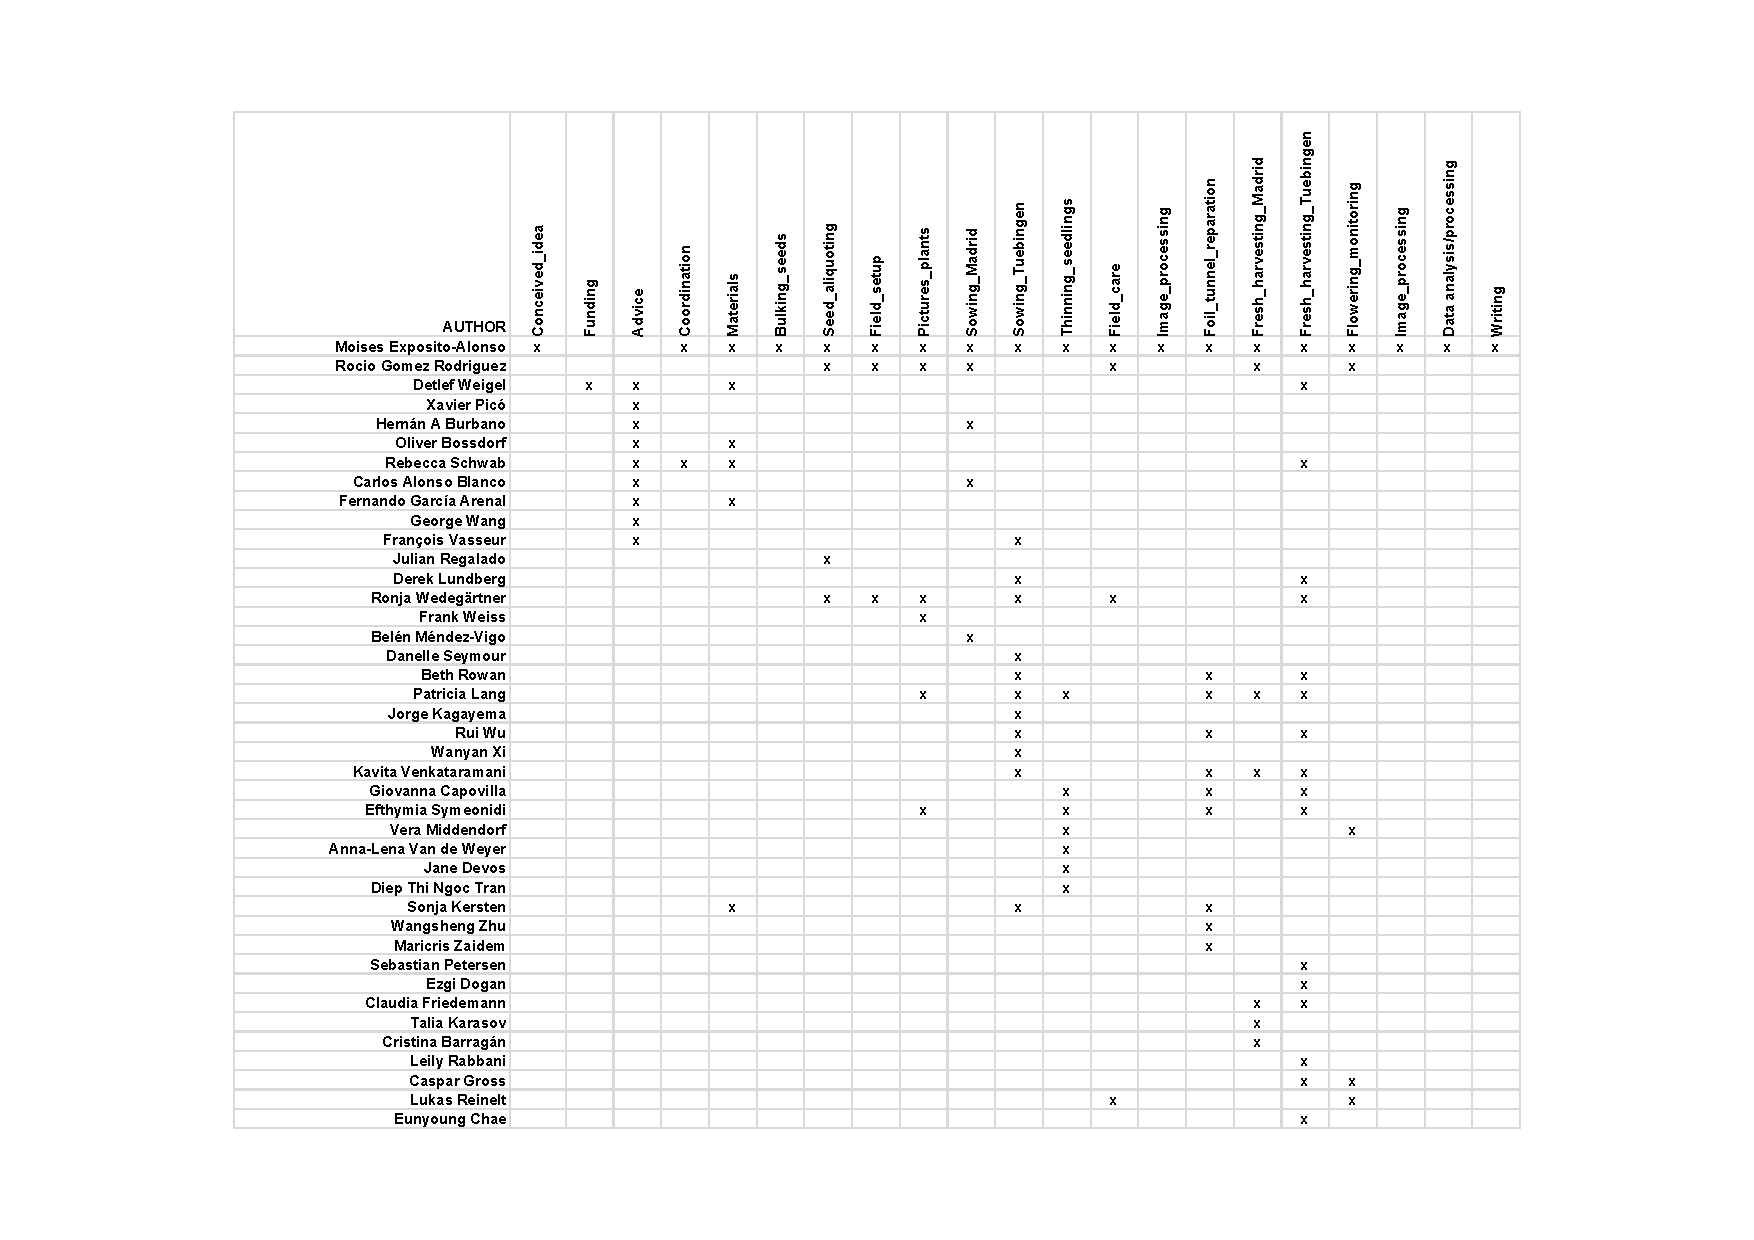
\includegraphics[width=7in]{../figs/People_paper.pdf}}

\section{References}\label{references}

\bibliography{references}

\pagebreak

\begin{figure}
    \centerline{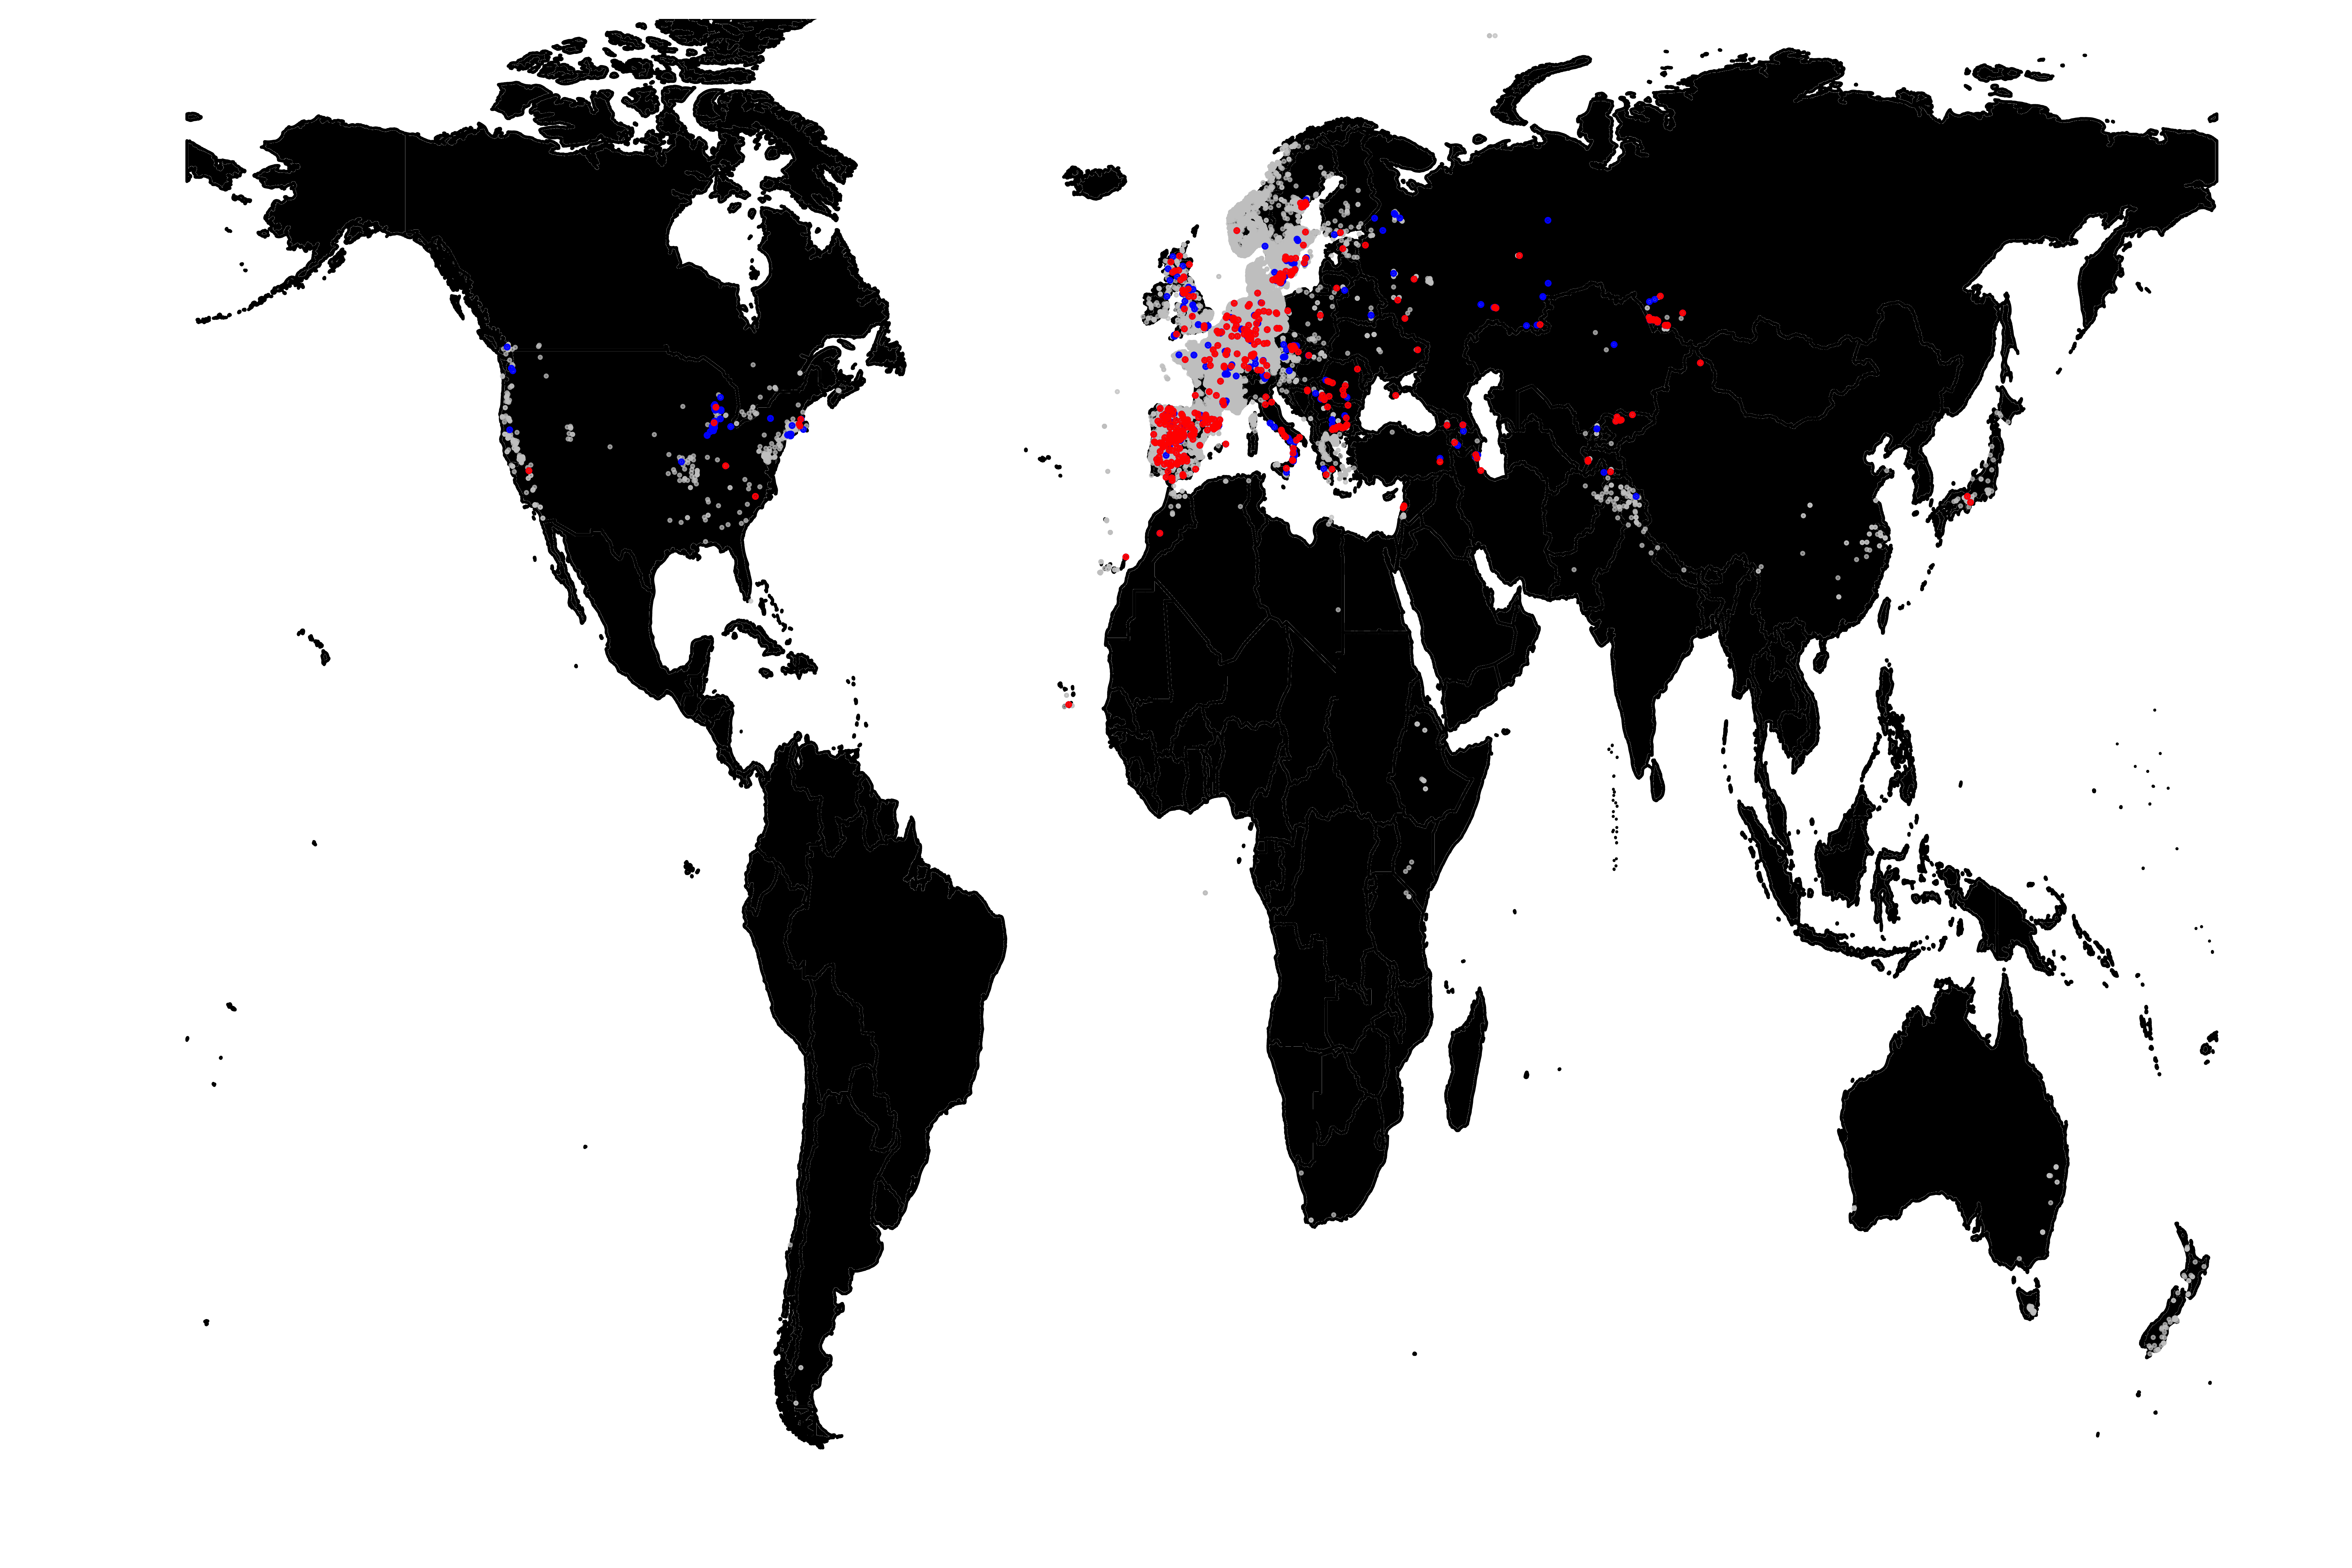
\includegraphics[width=5in]{../figs/Figure_gbif_field_occurrence_map.pdf}}
    \caption{ Locations of \textit{Arabidopsis thaliana} accessions used in this experiments (red), accessions included in the 1001 Genomes Project (blue), and all observations of the species in gbif.org}
    \label{fig:ecotypes}
\end{figure}

\begin{figure}
    \centering
    \begin{subfigure}[t]{0.45\textwidth}
        \centering
        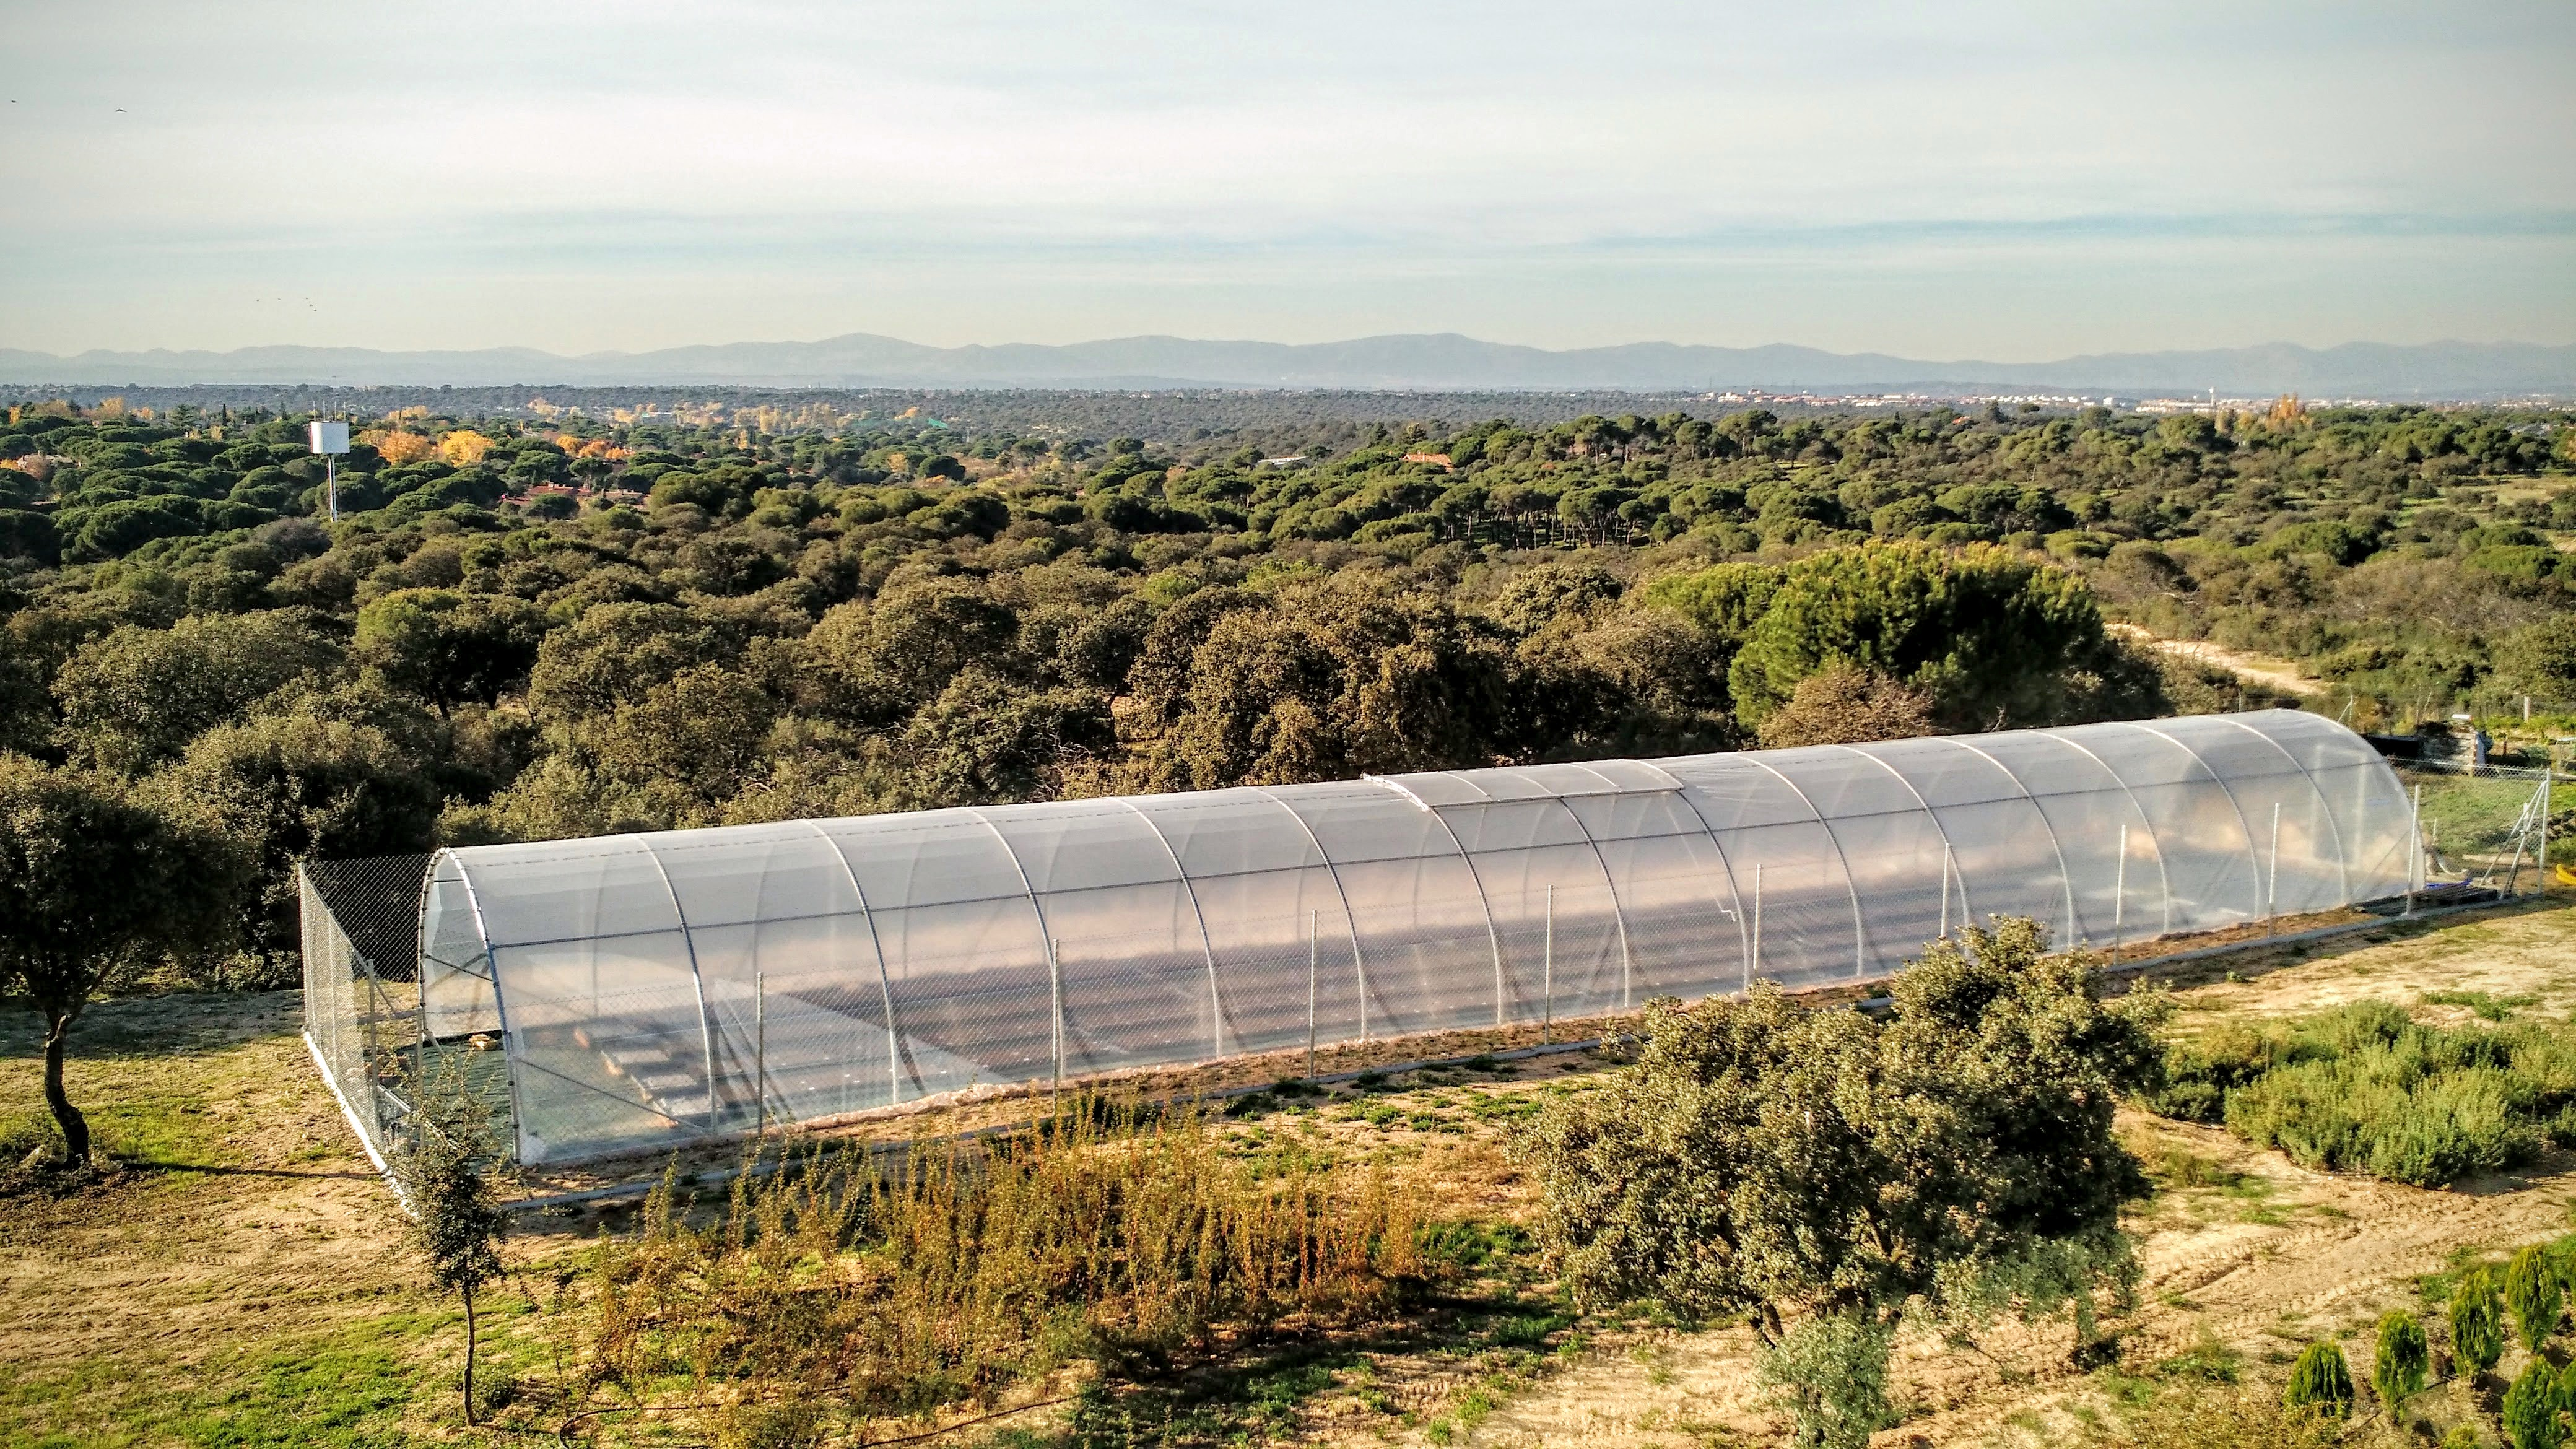
\includegraphics[width=\linewidth]{../figs/IMG_20151113_154250988.jpg}
        \caption{} \label{fig:aereal}
    \end{subfigure}
    \begin{subfigure}[t]{0.45\textwidth}
        \centering
        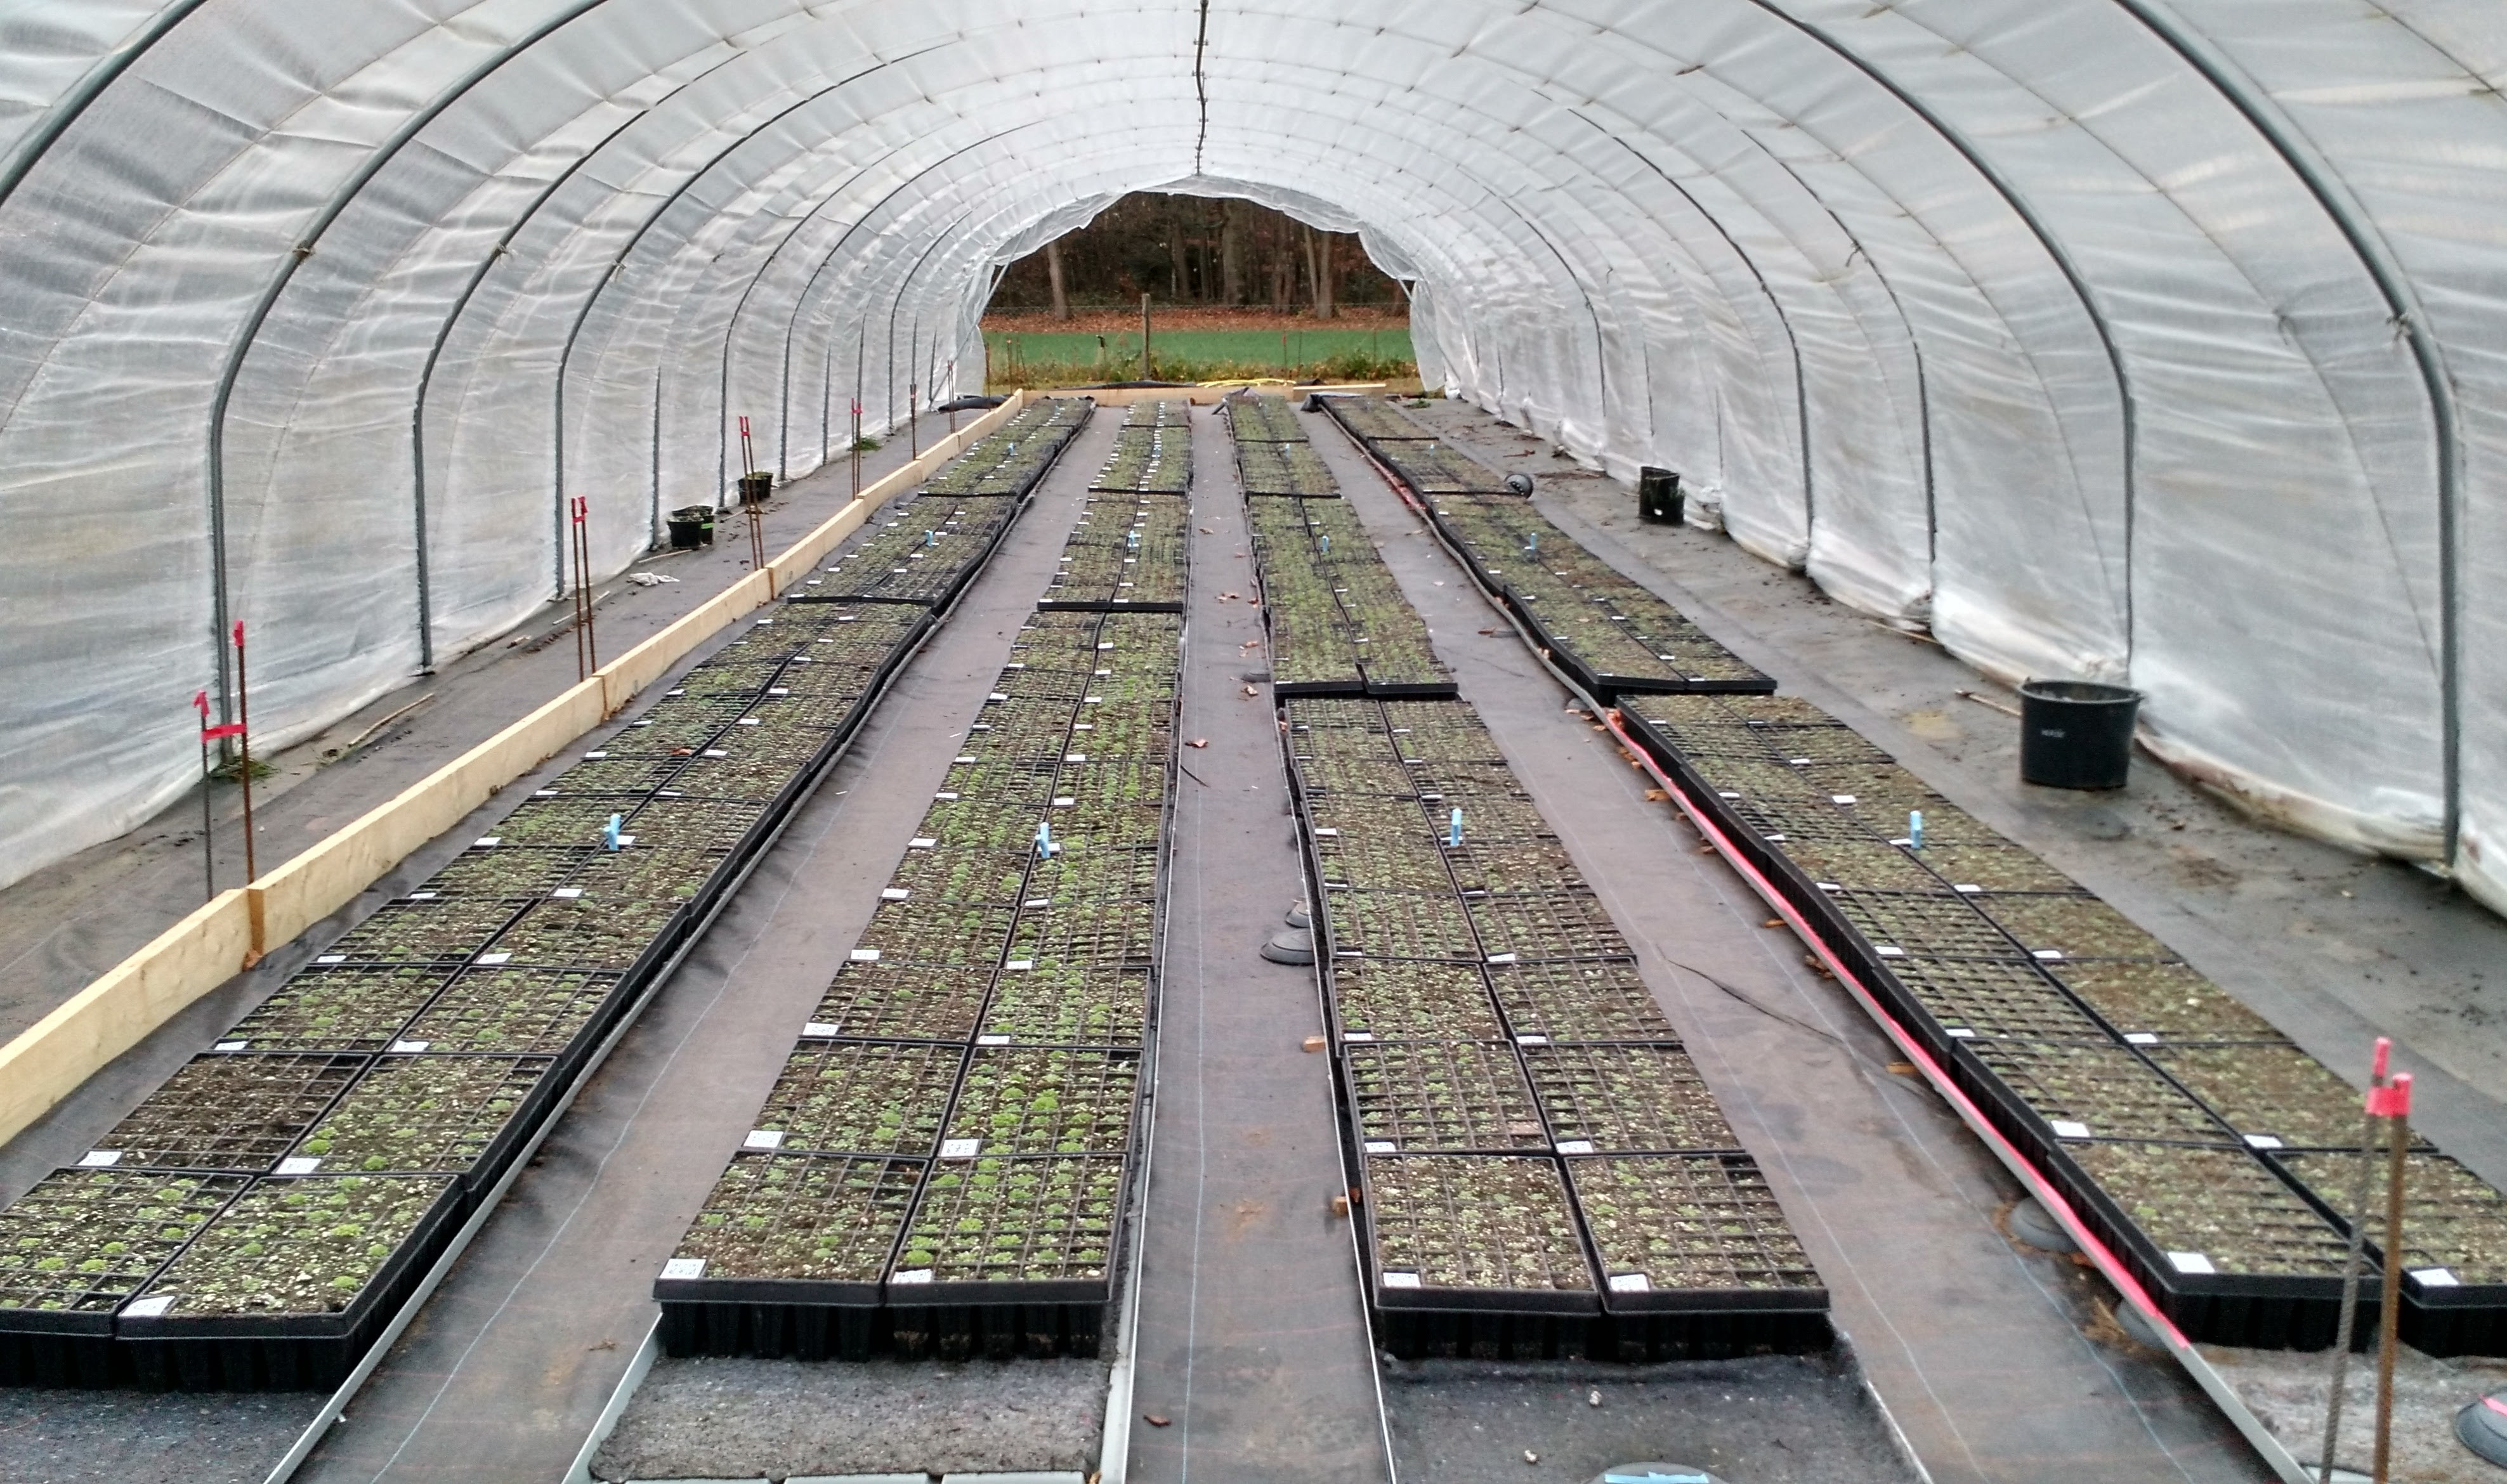
\includegraphics[width=\linewidth]{../figs/IMG_20151121_162359474_HDR.jpg}
        \caption{} \label{fig:inside}
    \end{subfigure}
     \caption{Aereal picture of foil tunnel setting in Madrid (\subref{fig:aereal}) and photo inside the foil tunnel in Tübingen (\subref{fig:inside}).}
\end{figure}

\begin{figure}
 \centerline{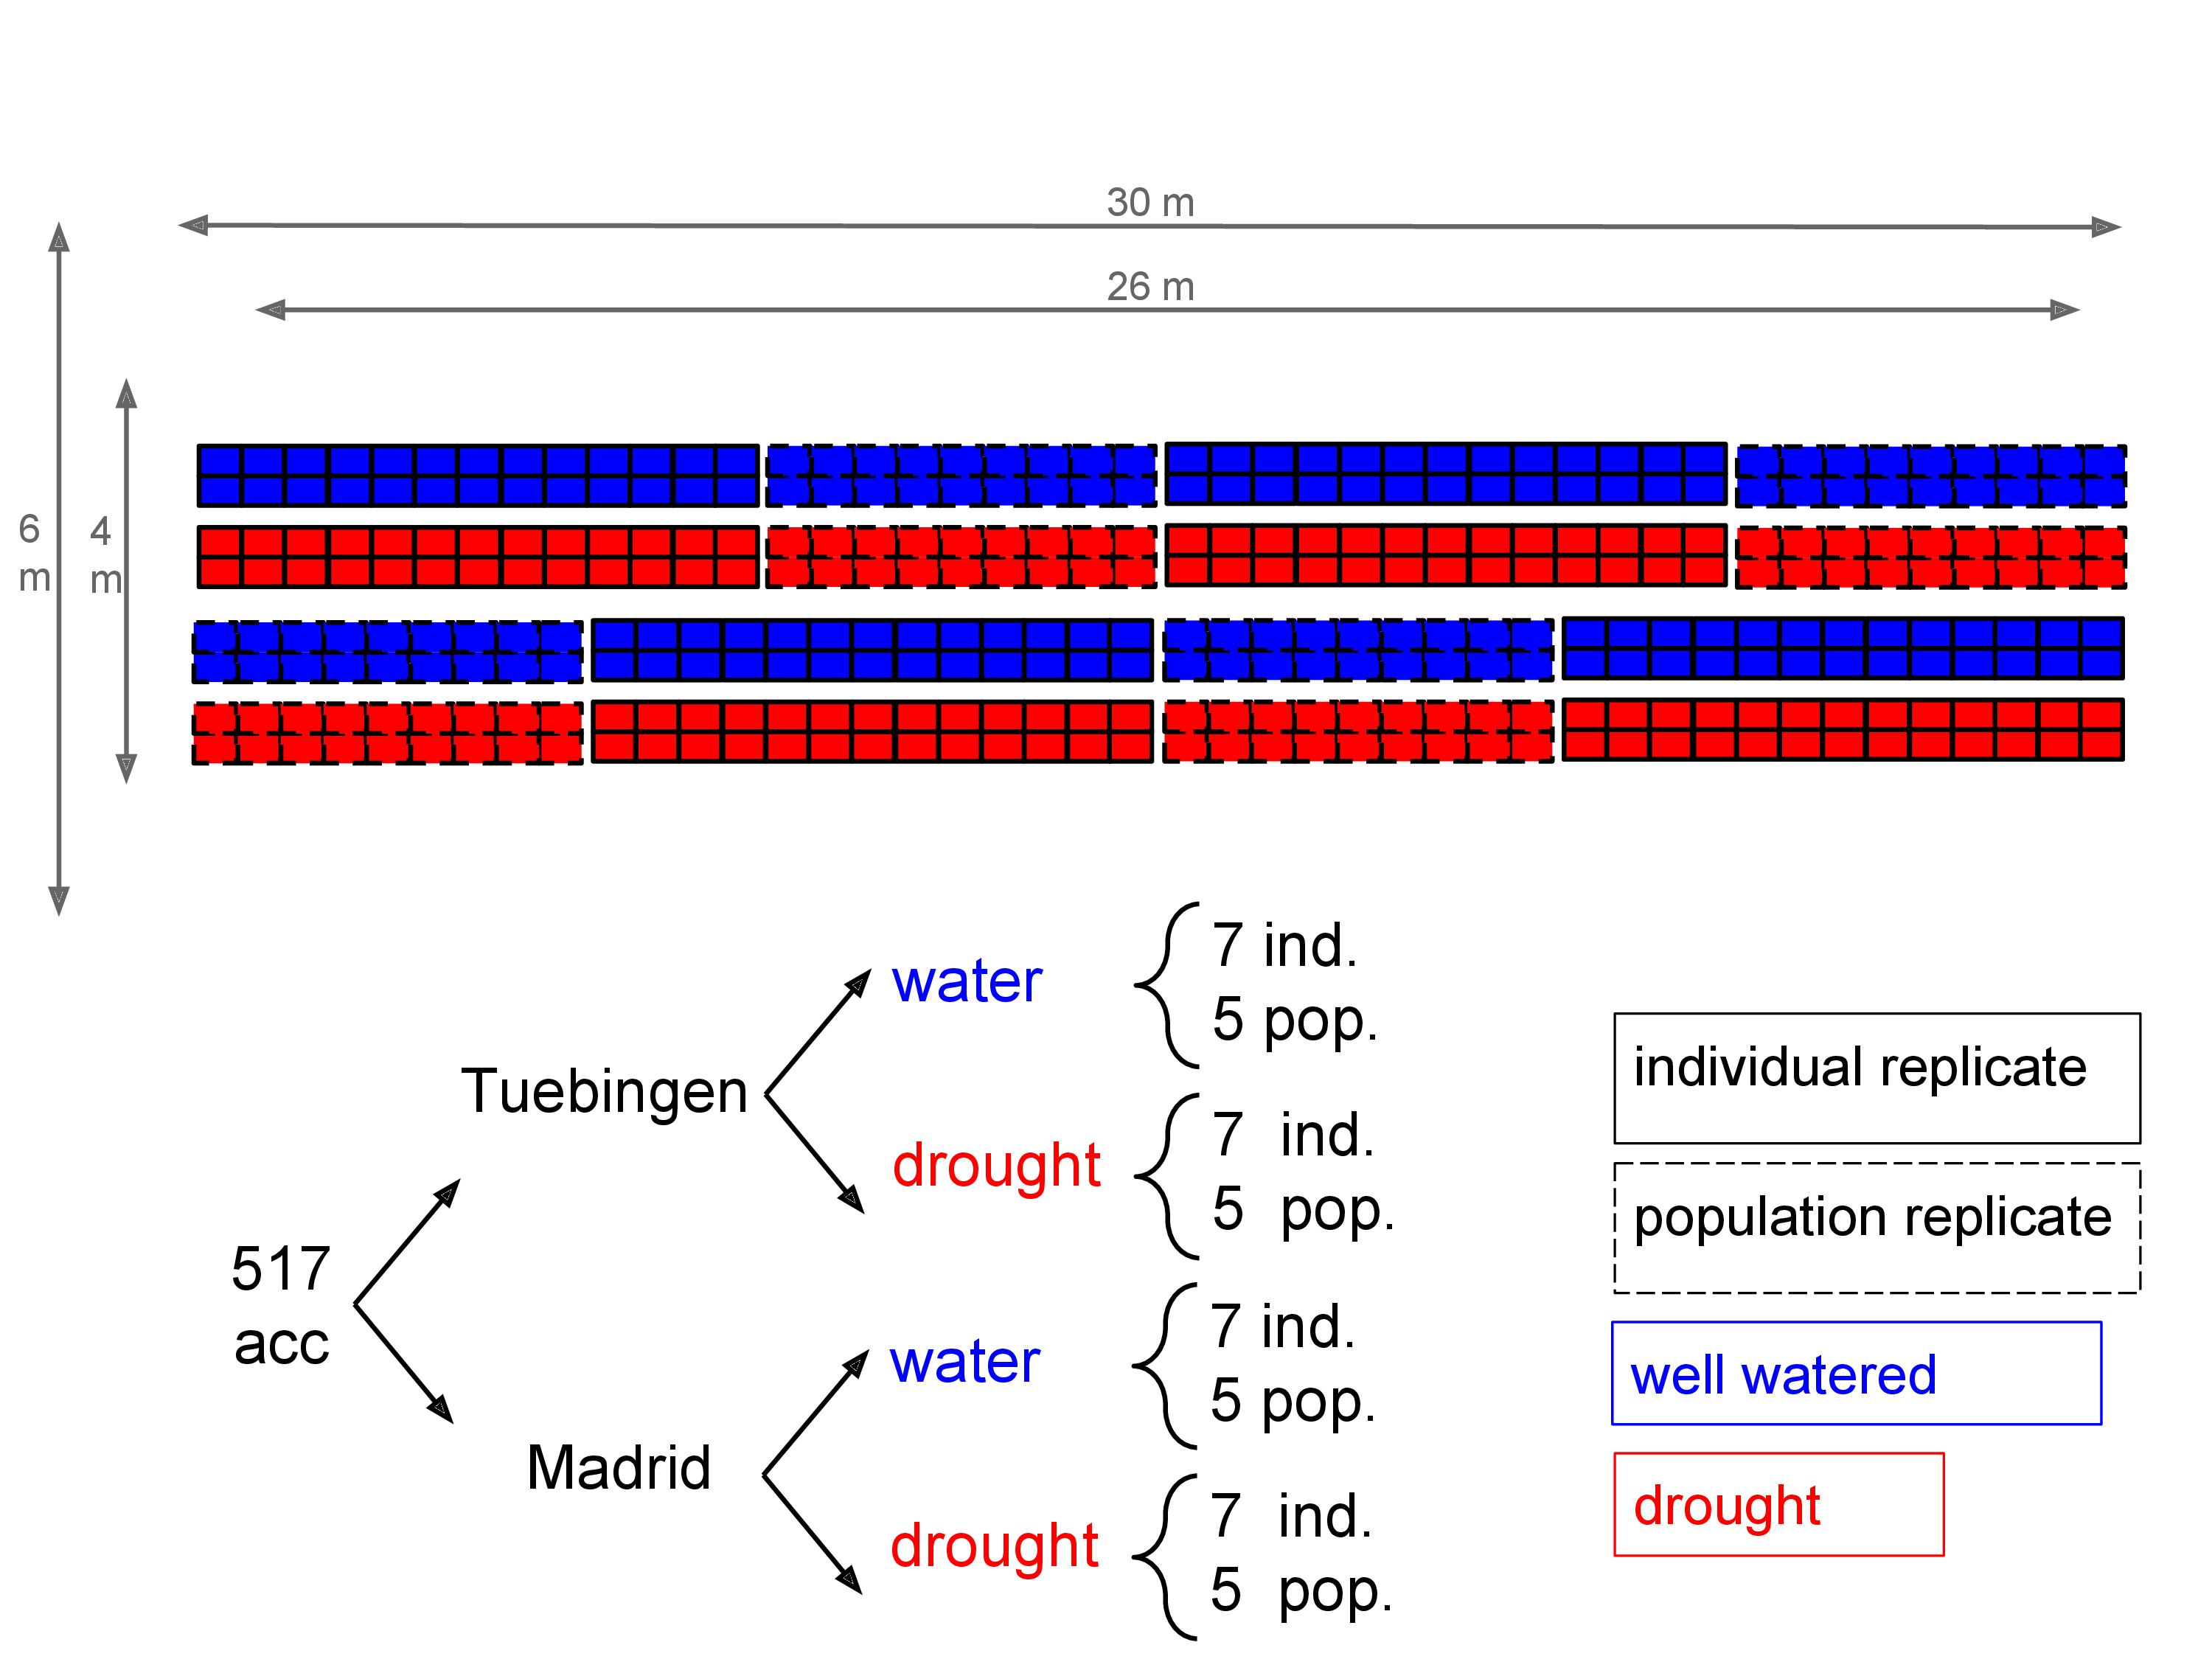
\includegraphics[width=5in]{../figs/Figure_field_spatial_distribution.pdf}}
    \caption{ Design and spatial distribution of blocks and replicates}
    \label{fig:blocks}
\end{figure}

\begin{figure}
  \centering
      \begin{subfigure}[b]{0.25\textwidth}
        \centering
        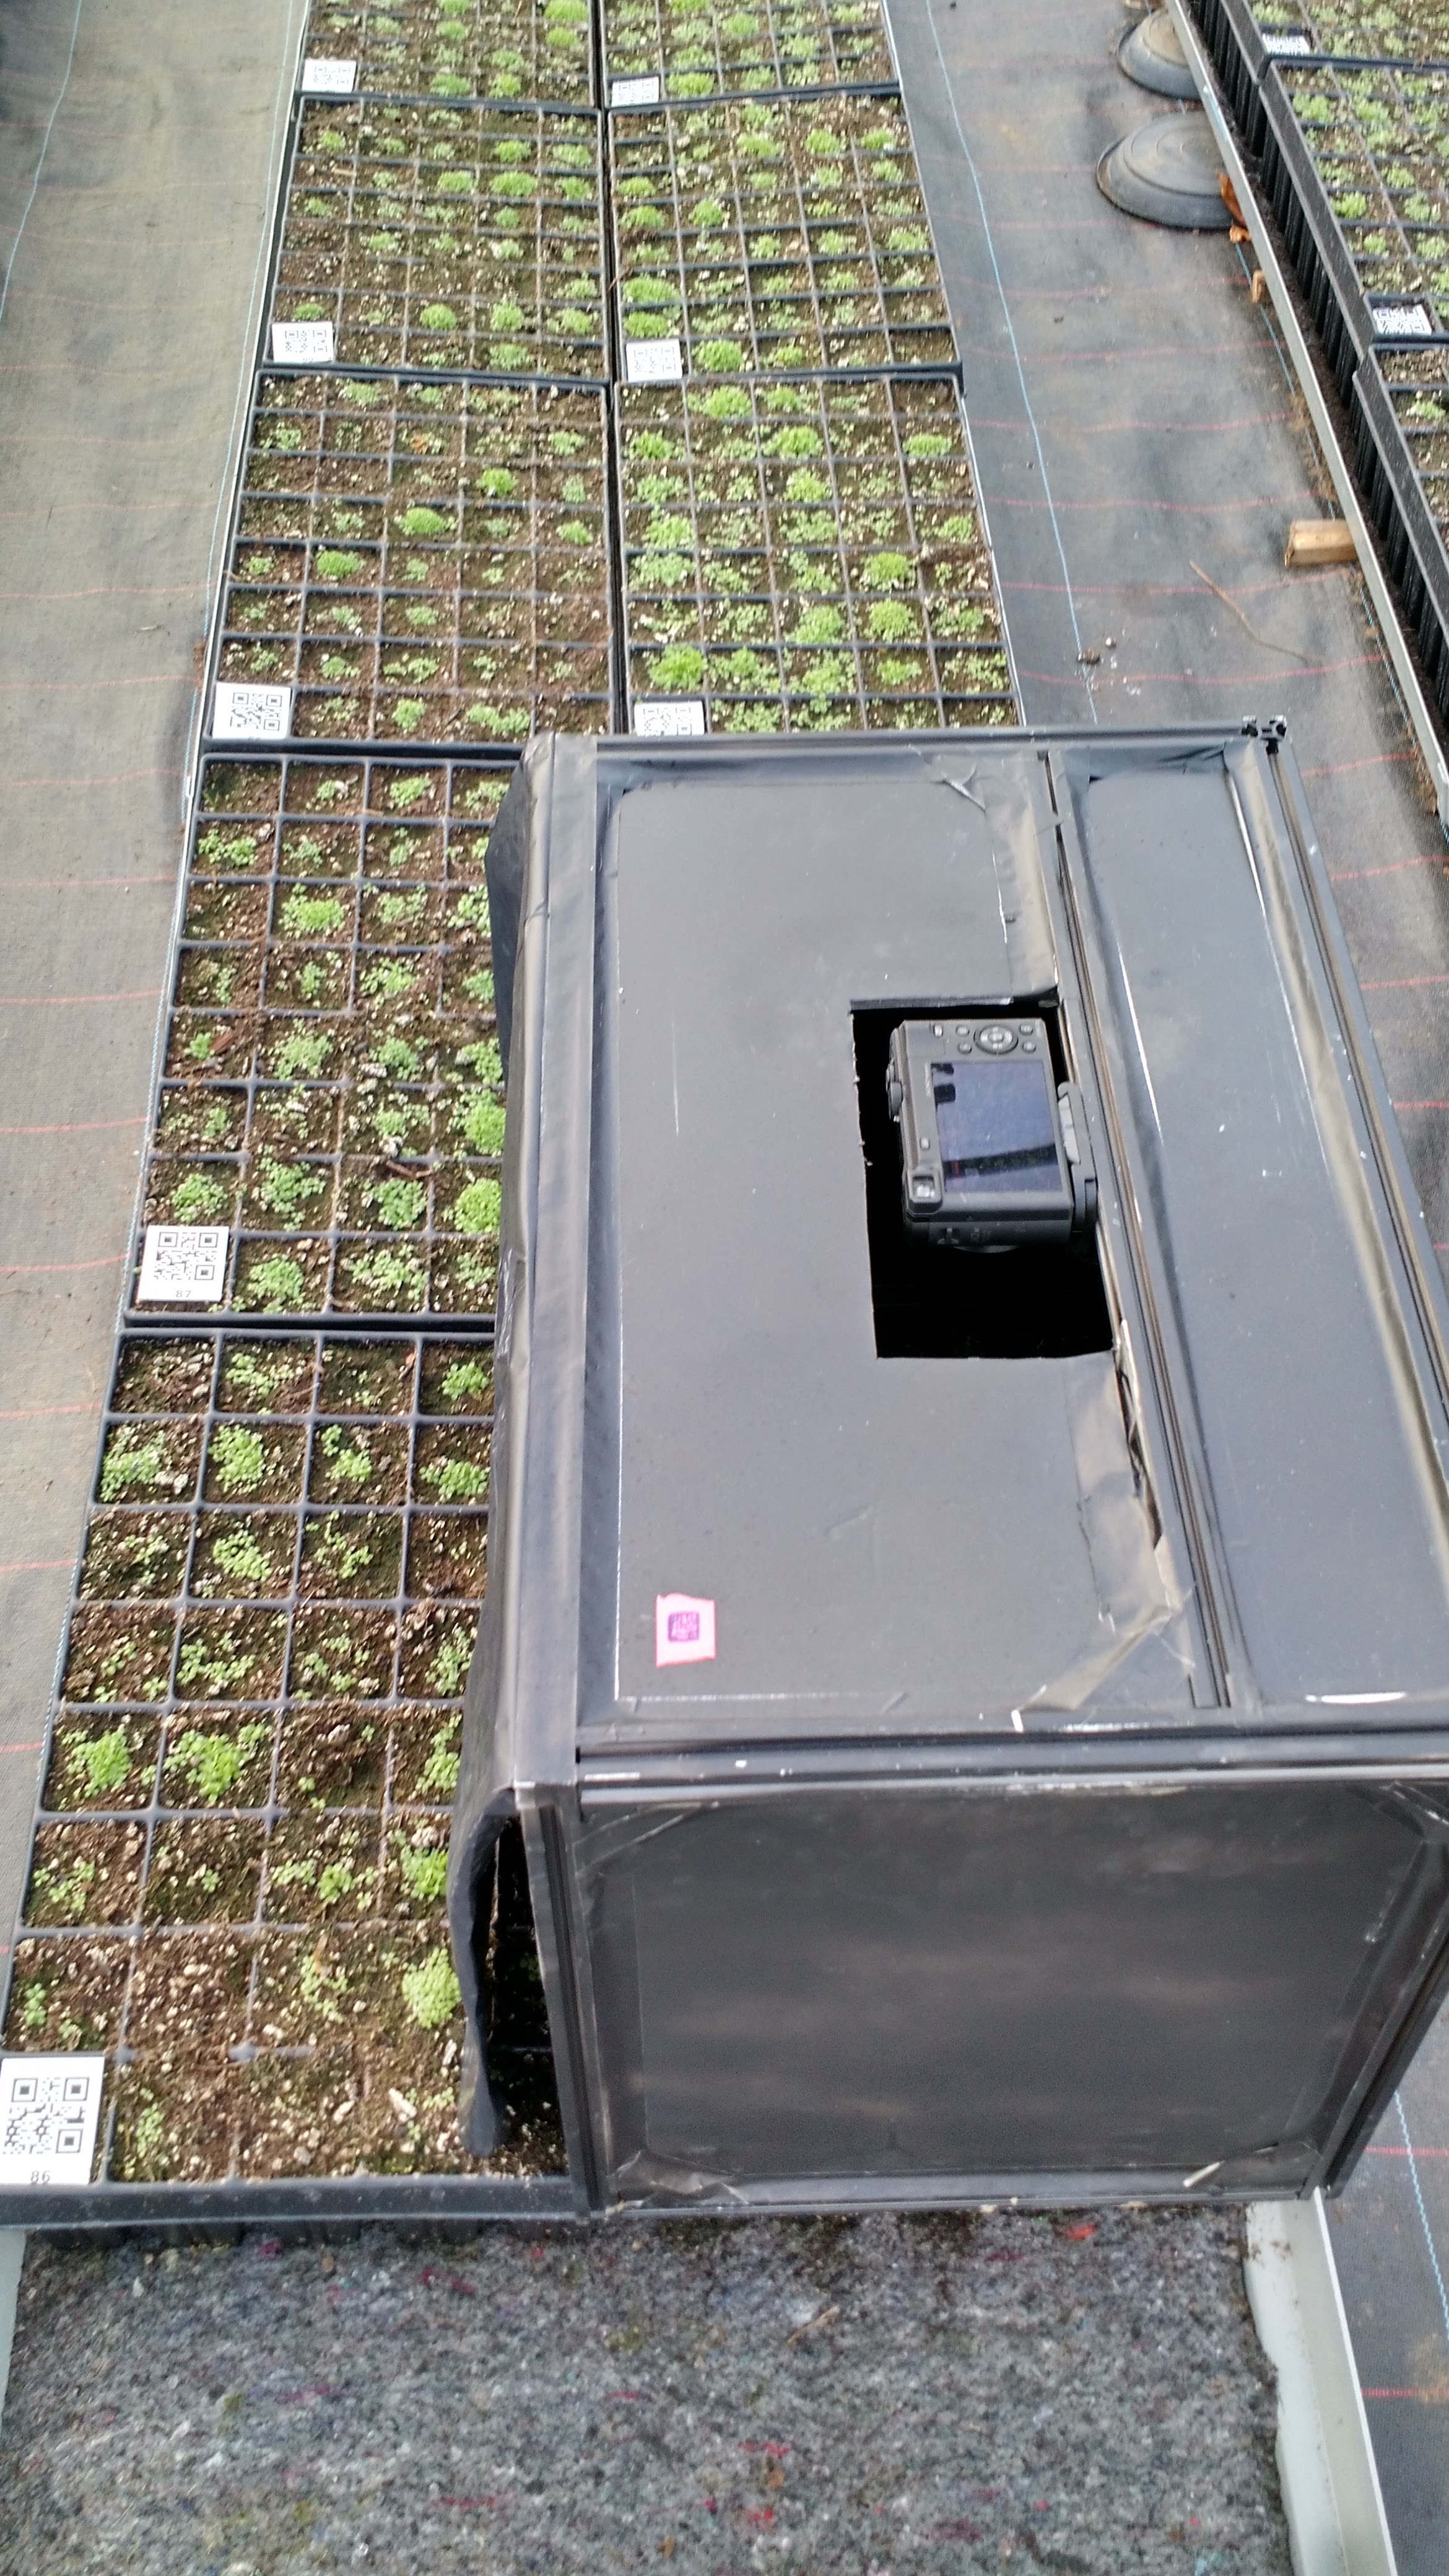
\includegraphics[width=\linewidth]{../figs/IMG_20151123_151811961_HDR.jpg}
        \caption{} \label{fig:photobox}
    \end{subfigure}
    \begin{subfigure}[b]{0.6\textwidth}
        \centering
        \includegraphics[width=\linewidth]{../figs/Figure_example_trays.pdf}
        \caption{} \label{fig:exampletrays}
    \end{subfigure}
    \caption{ Customized black box for image acquisition (\subref{fig:photobox}) and example trays  (\subref{fig:exampletrays})  of the four watering x replicate type combinations: low watering and population replicate (upper-left), high watering and population replicate (upper-right), low watering and individual replicate (lower-left), high watering and individual replicate (lower-right). }
    \label{fig:trays}
\end{figure}

\begin{figure}
    \centering
    \begin{subfigure}[t]{0.8\textwidth}
        \centering
        \includegraphics[width=\linewidth]{../figs/P1030542.JPG}
        \caption{} \label{fig:rawseg}
    \end{subfigure}
    \begin{subfigure}[t]{0.45\textwidth}
        \centering
        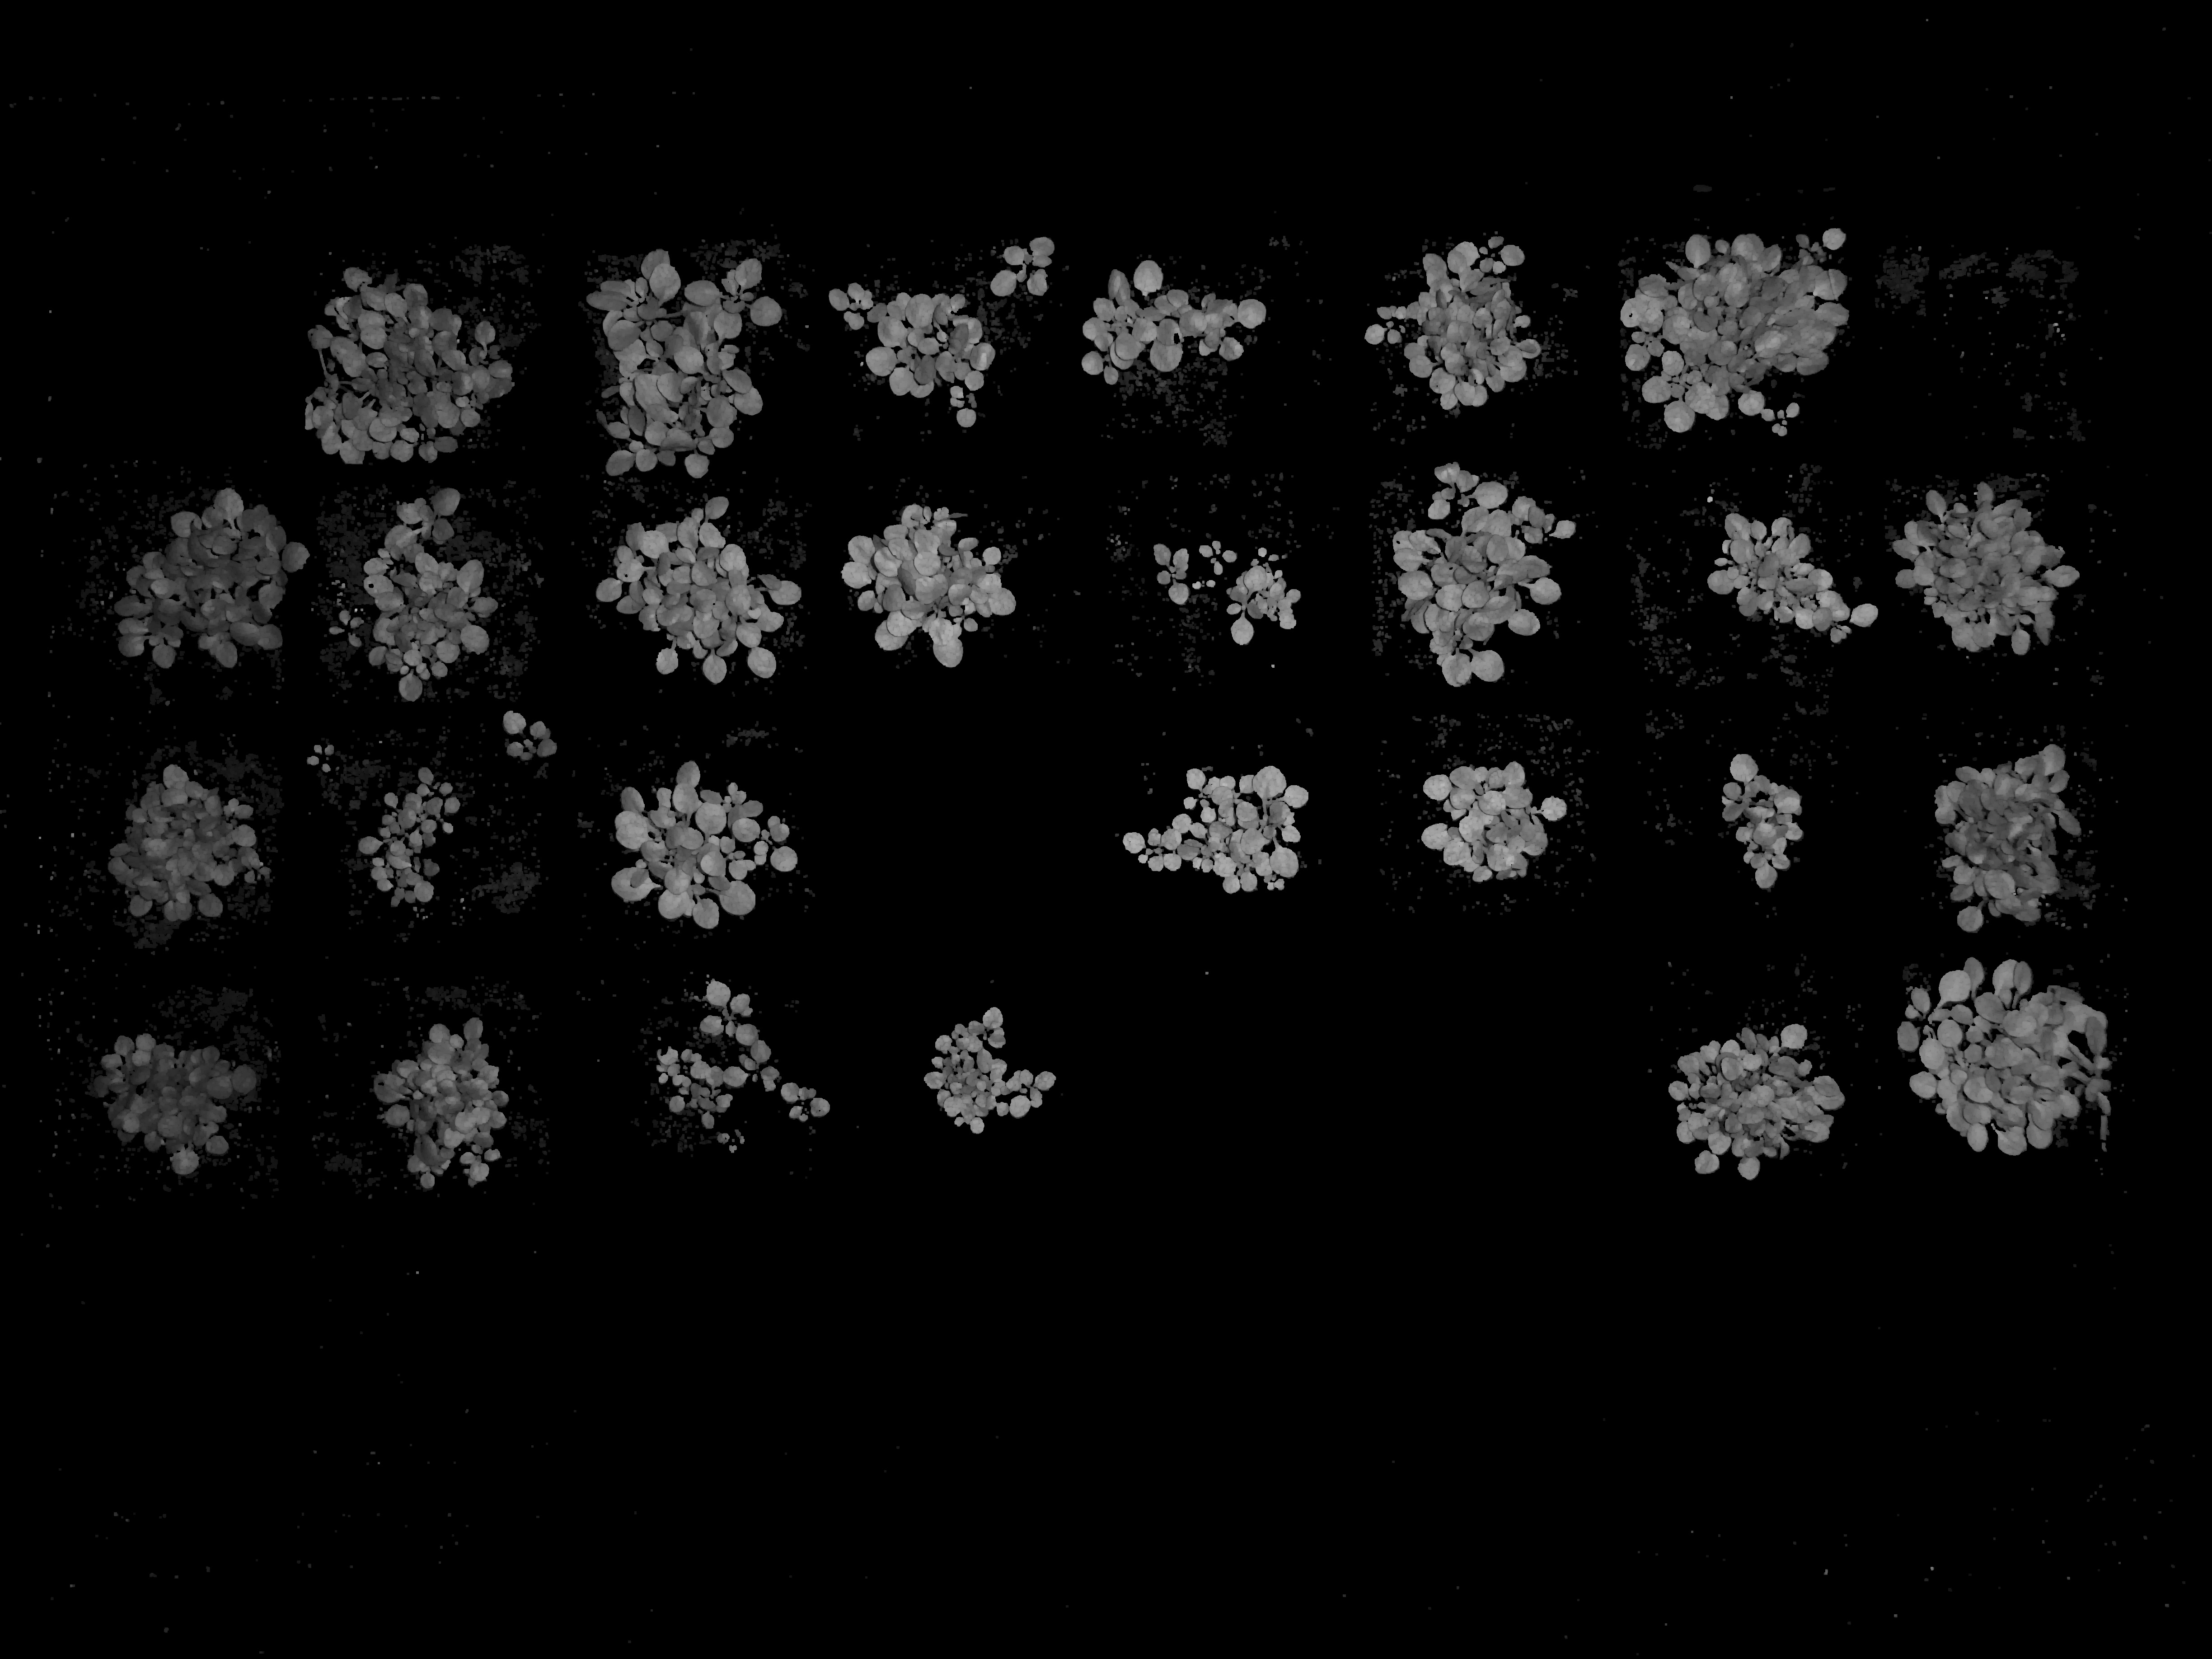
\includegraphics[width=\linewidth]{../figs/P1030542.JPG_seggreen.jpeg}
        \caption{} \label{fig:greenexample}
    \end{subfigure}
    \begin{subfigure}[t]{0.45\textwidth}
        \centering
        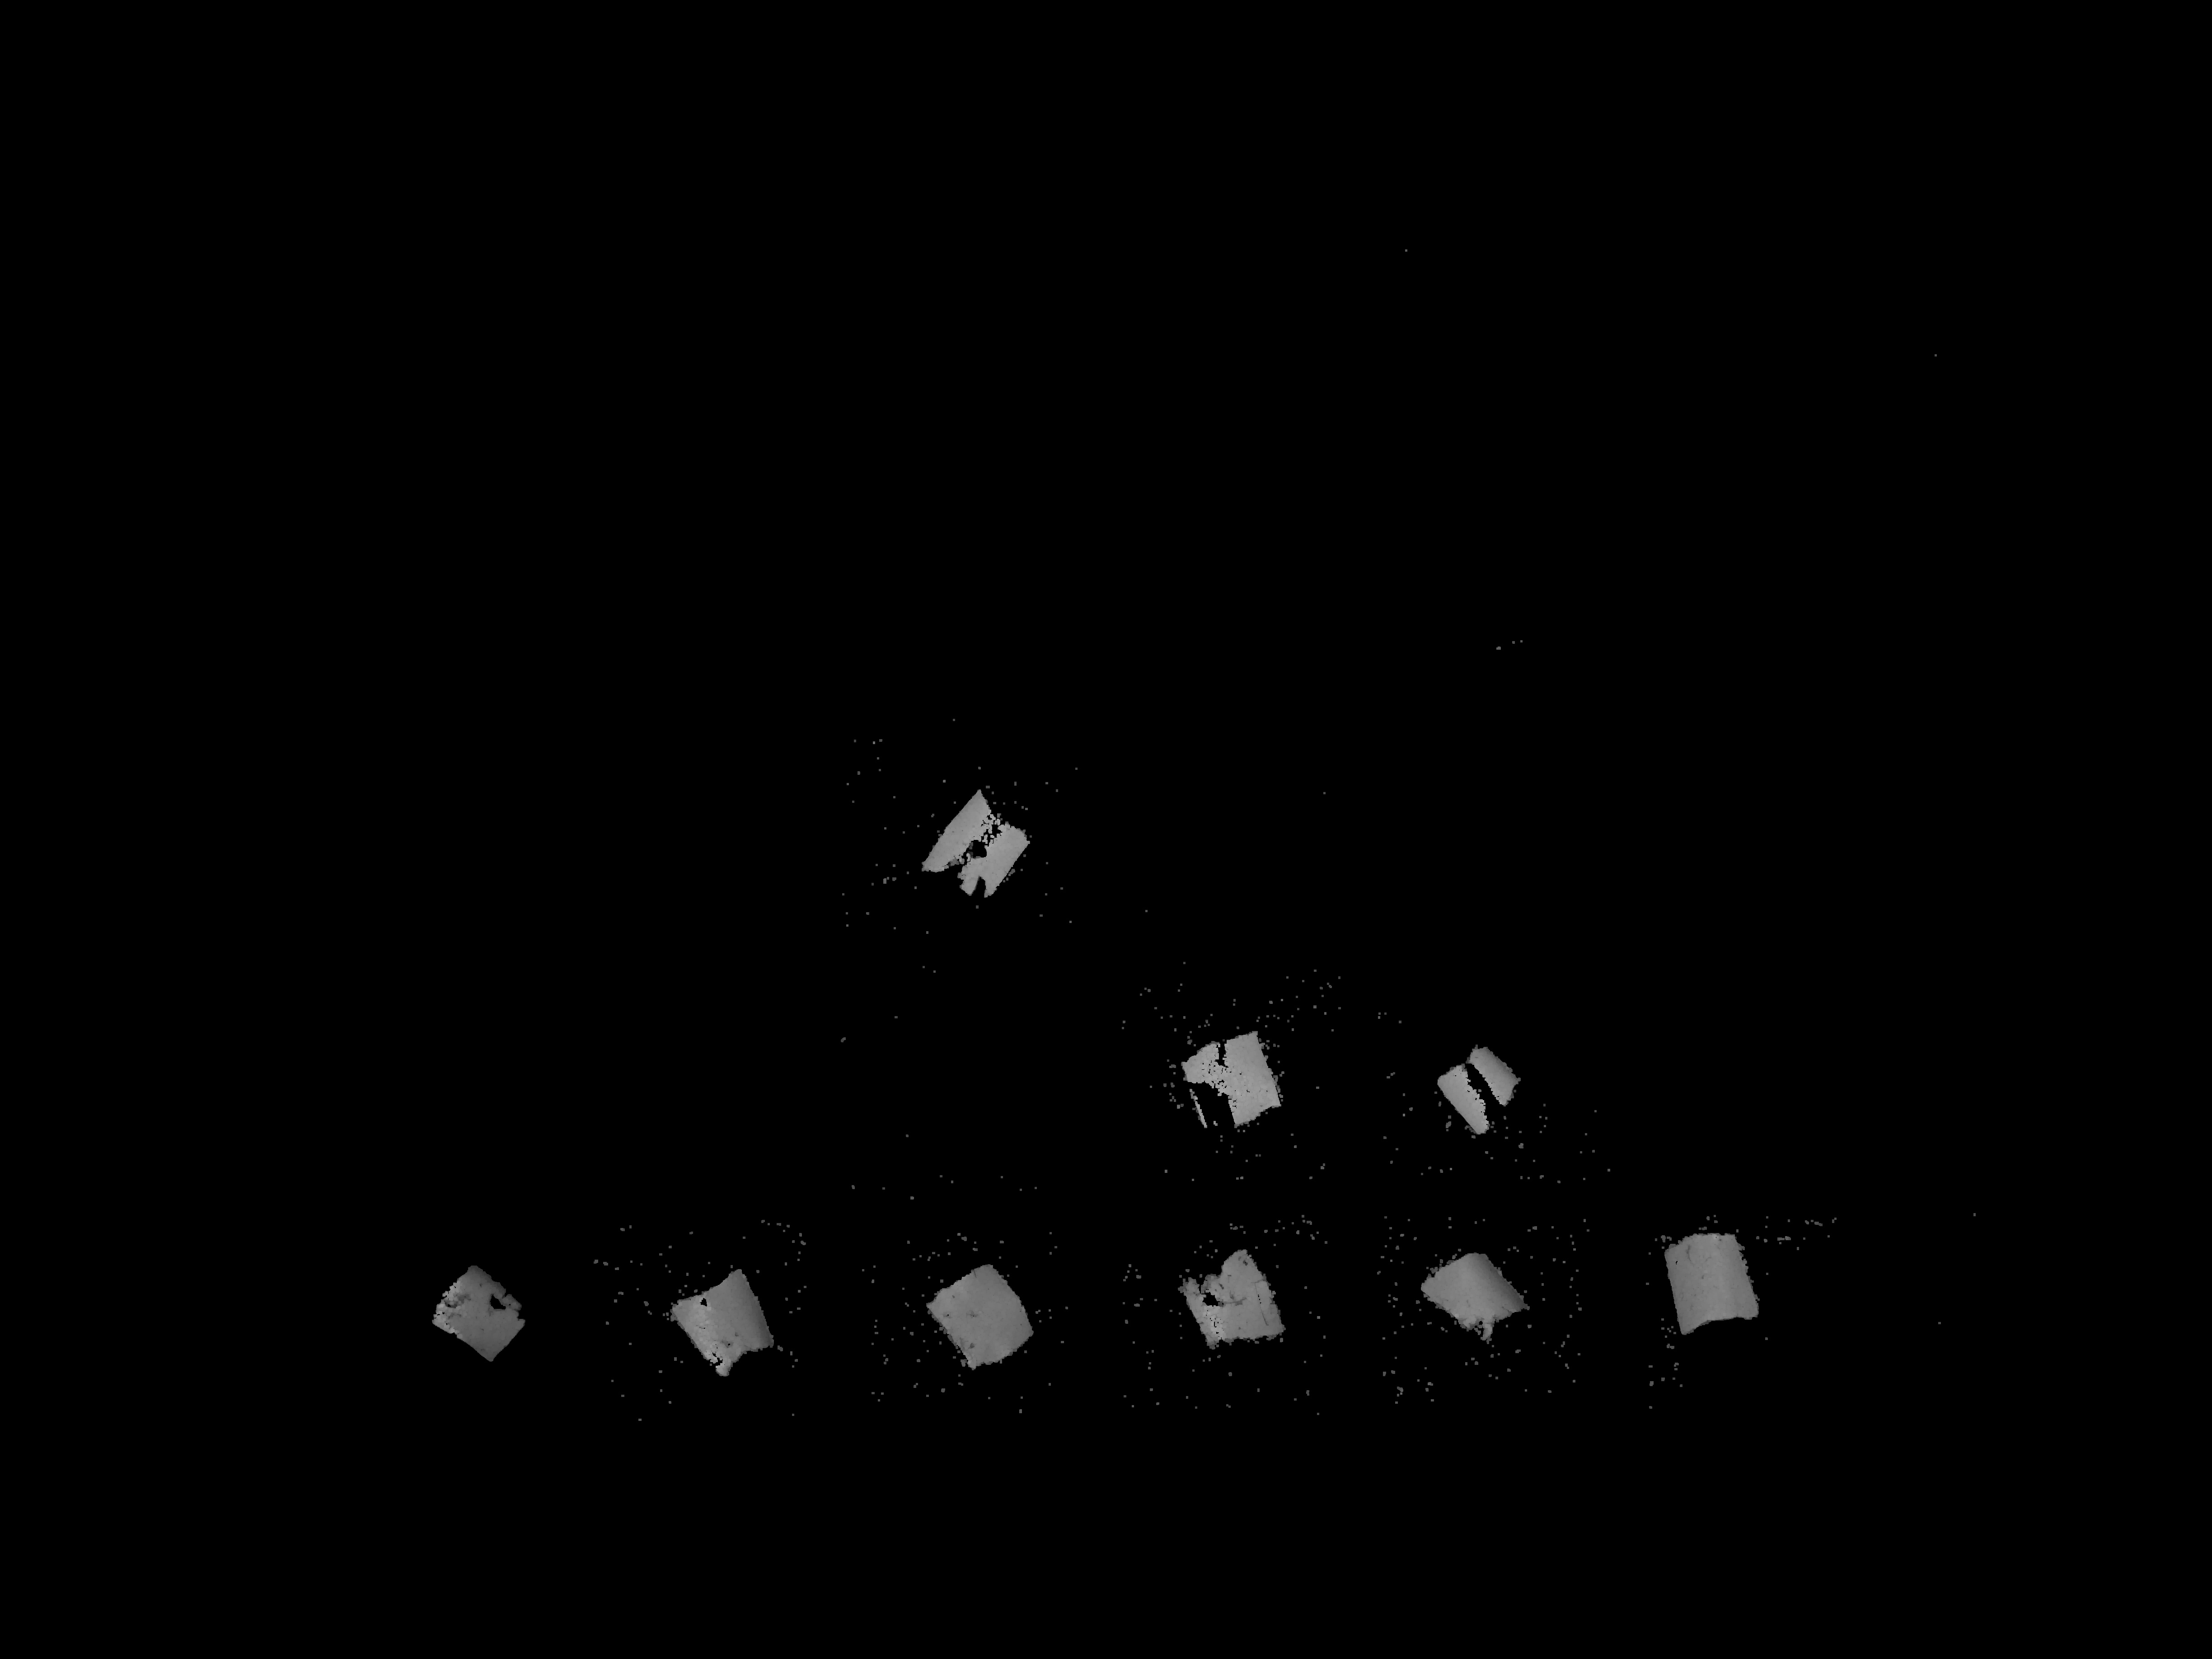
\includegraphics[width=\linewidth]{../figs/P1030542.JPG_seggreenred.jpeg}
        \caption{} \label{fig:redexample}
    \end{subfigure}
    \caption{Example segmentation results from raw image (\subref{fig:rawseg}) to green (\subref{fig:greenexample})  and red (\subref{fig:redexample}) pixels only.}
    \label{fig:segmentation}
\end{figure}

\begin{figure}
    \centering
    \begin{subfigure}[t]{0.8\textwidth}
        \centering
        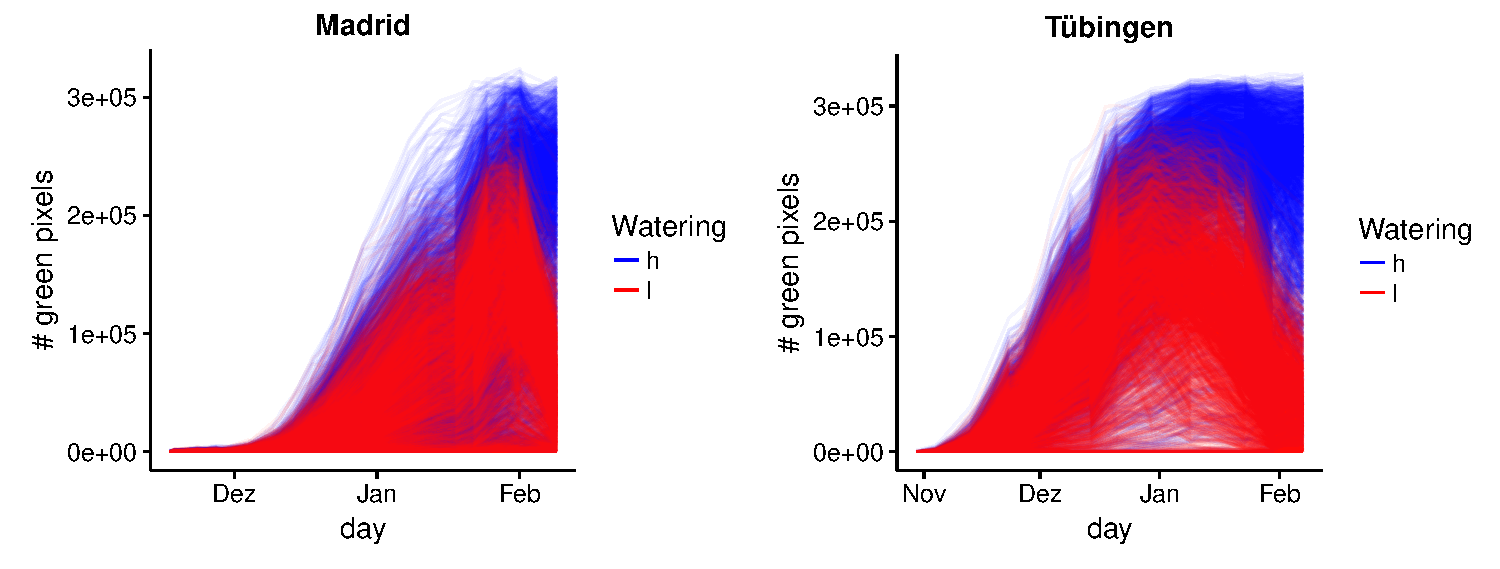
\includegraphics[width=6in]{../figs/Figure_green_trajectory.pdf}
        \caption{} \label{fig:growth}
    \end{subfigure}
        \begin{subfigure}[t]{0.8\textwidth}
        \centering
        \centerline{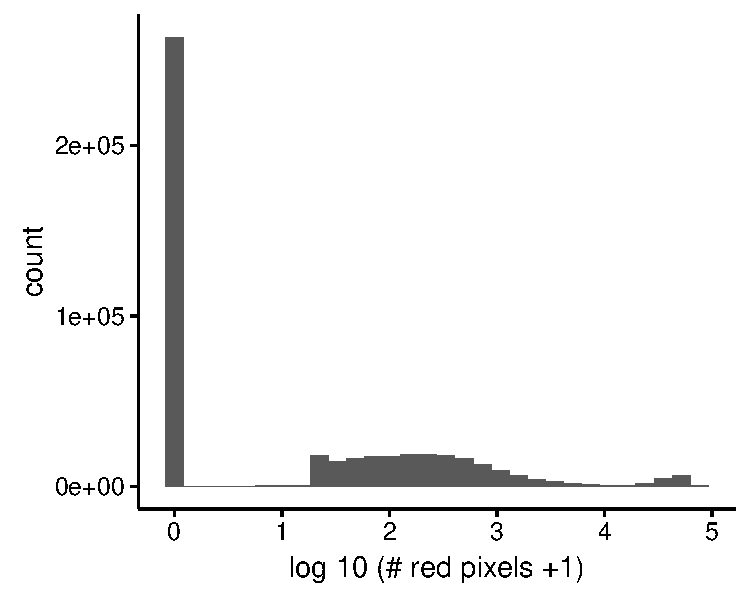
\includegraphics[width=3in]{../figs/Figure_redcount_histogram.pdf}}
        \caption{} \label{fig:red}
    \end{subfigure}
    \caption{Trajectories per pot of number of green pixels for Madrid and Tübingen (\subref{fig:growth}). Distribution of the number of red pixels per pot summed over different time frames (\subref{fig:red}) and the heuristically chosen threshold to define whether the pot actually had a red label(red vertical line).}
    \label{fig:pixels}
\end{figure}

\begin{figure}
    \centerline{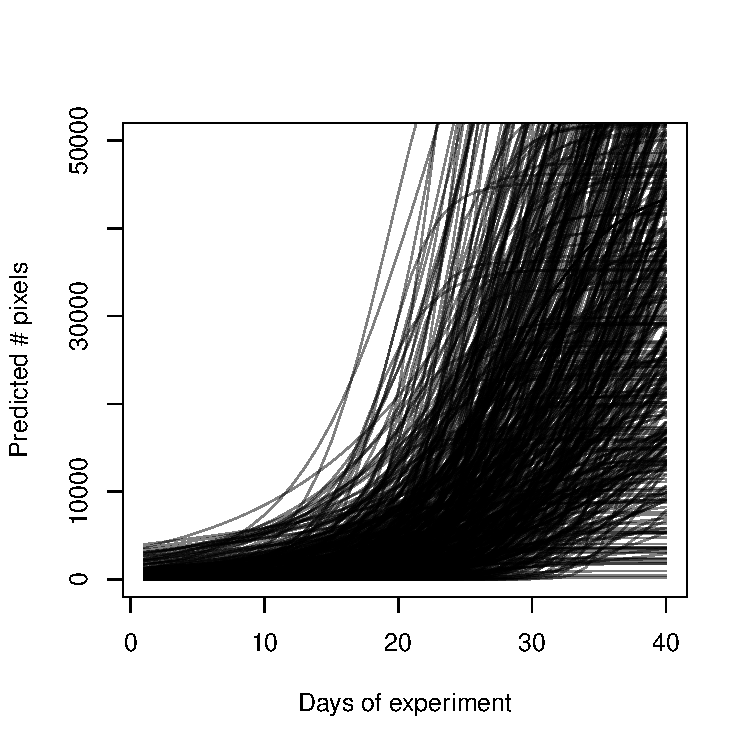
\includegraphics[width=5in]{../figs/Figure_growth_trajectories.pdf}}
    \caption{ Randomly selected growth trajectories from 1000 pots}
    \label{fig:trajectories}
\end{figure}

\begin{figure}
    \centerline{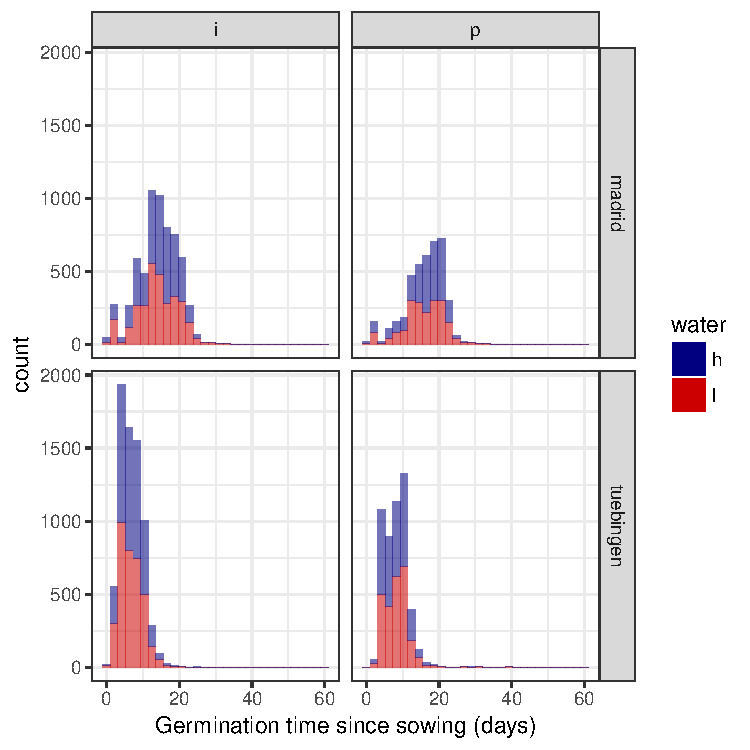
\includegraphics[width=5in]{../figs/Figure_germination_distribution.pdf}}
    \caption{ Distribution of germination times }
    \label{fig:germination}
\end{figure}

\begin{figure}
    \centerline{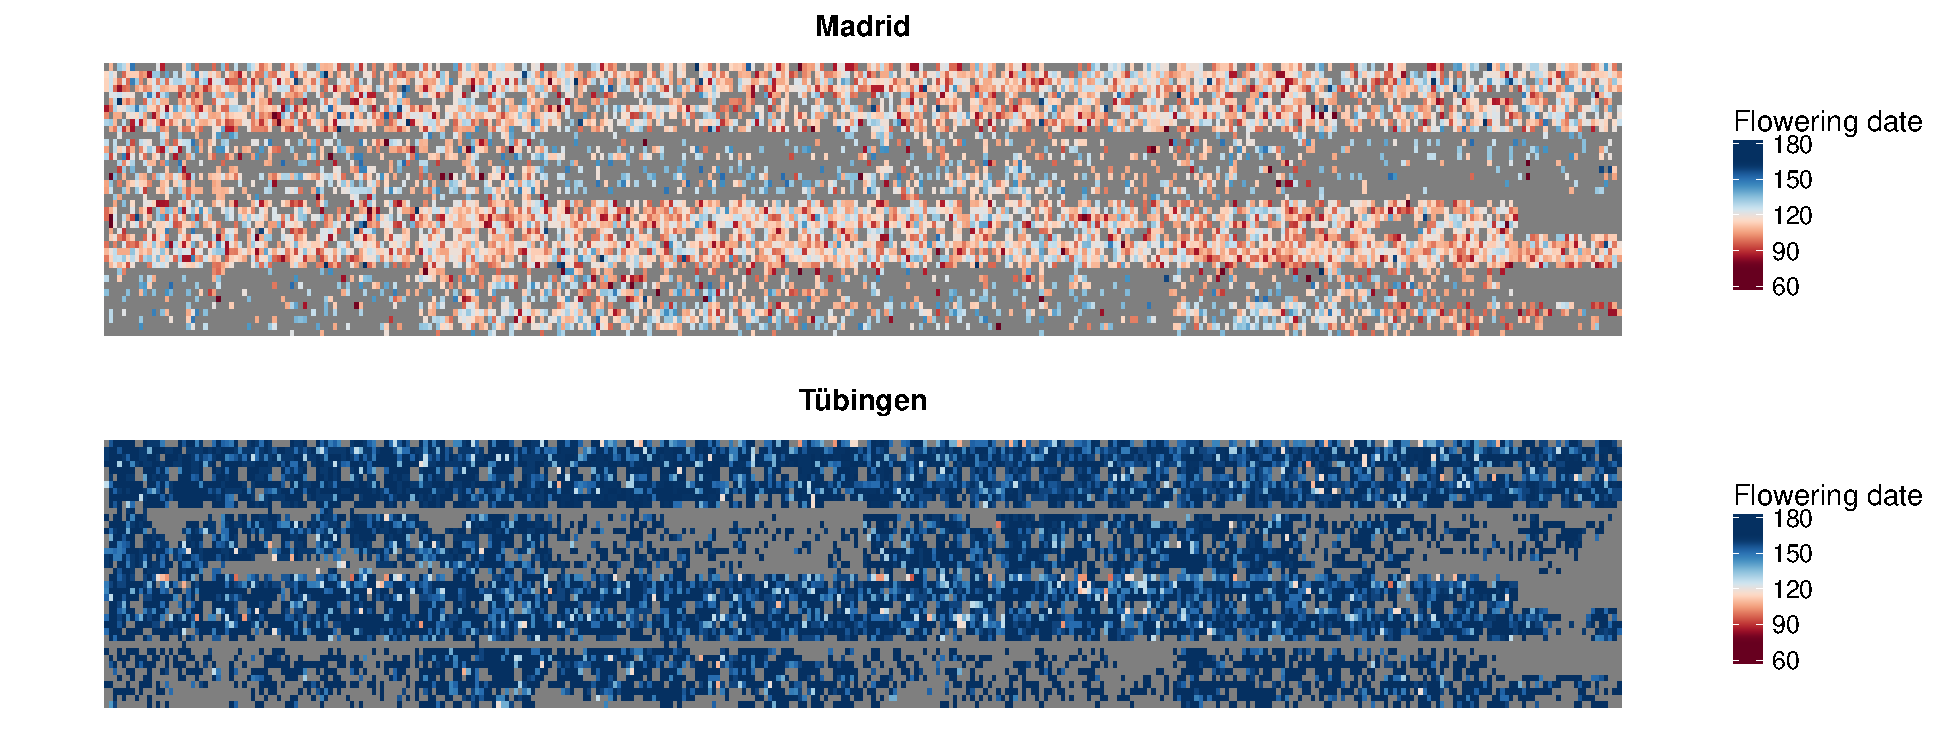
\includegraphics[width=6in]{../figs/Figure_raw_flowering.pdf}}
    \caption{ Days from sowing to flowering in the same spatial distribution as Fig. \ref{fig:blocks}}
    \label{fig:flowerraw}
\end{figure}

\begin{figure}
    \centerline{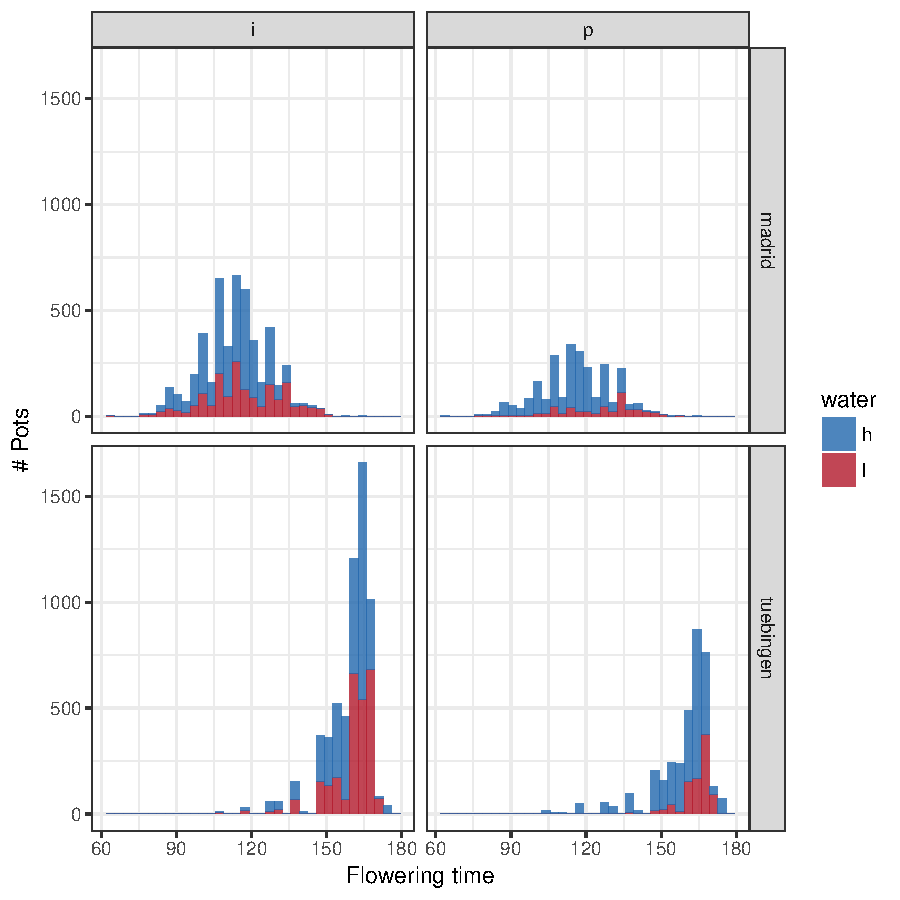
\includegraphics[width=5in]{../figs/Figure_flowering_distribution.pdf}}
    \caption{ Distribution of time since sowing date until flowering}
    \label{fig:flowerdistribution}
\end{figure}

\begin{figure}
    \centering
    \begin{subfigure}[t]{0.8\textwidth}
        \centering
        \includegraphics[width=\linewidth]{../figs/P1060902.JPG}
        \caption{} \label{fig:original}
    \end{subfigure}
    \begin{subfigure}[t]{0.45\textwidth}
        \centering
        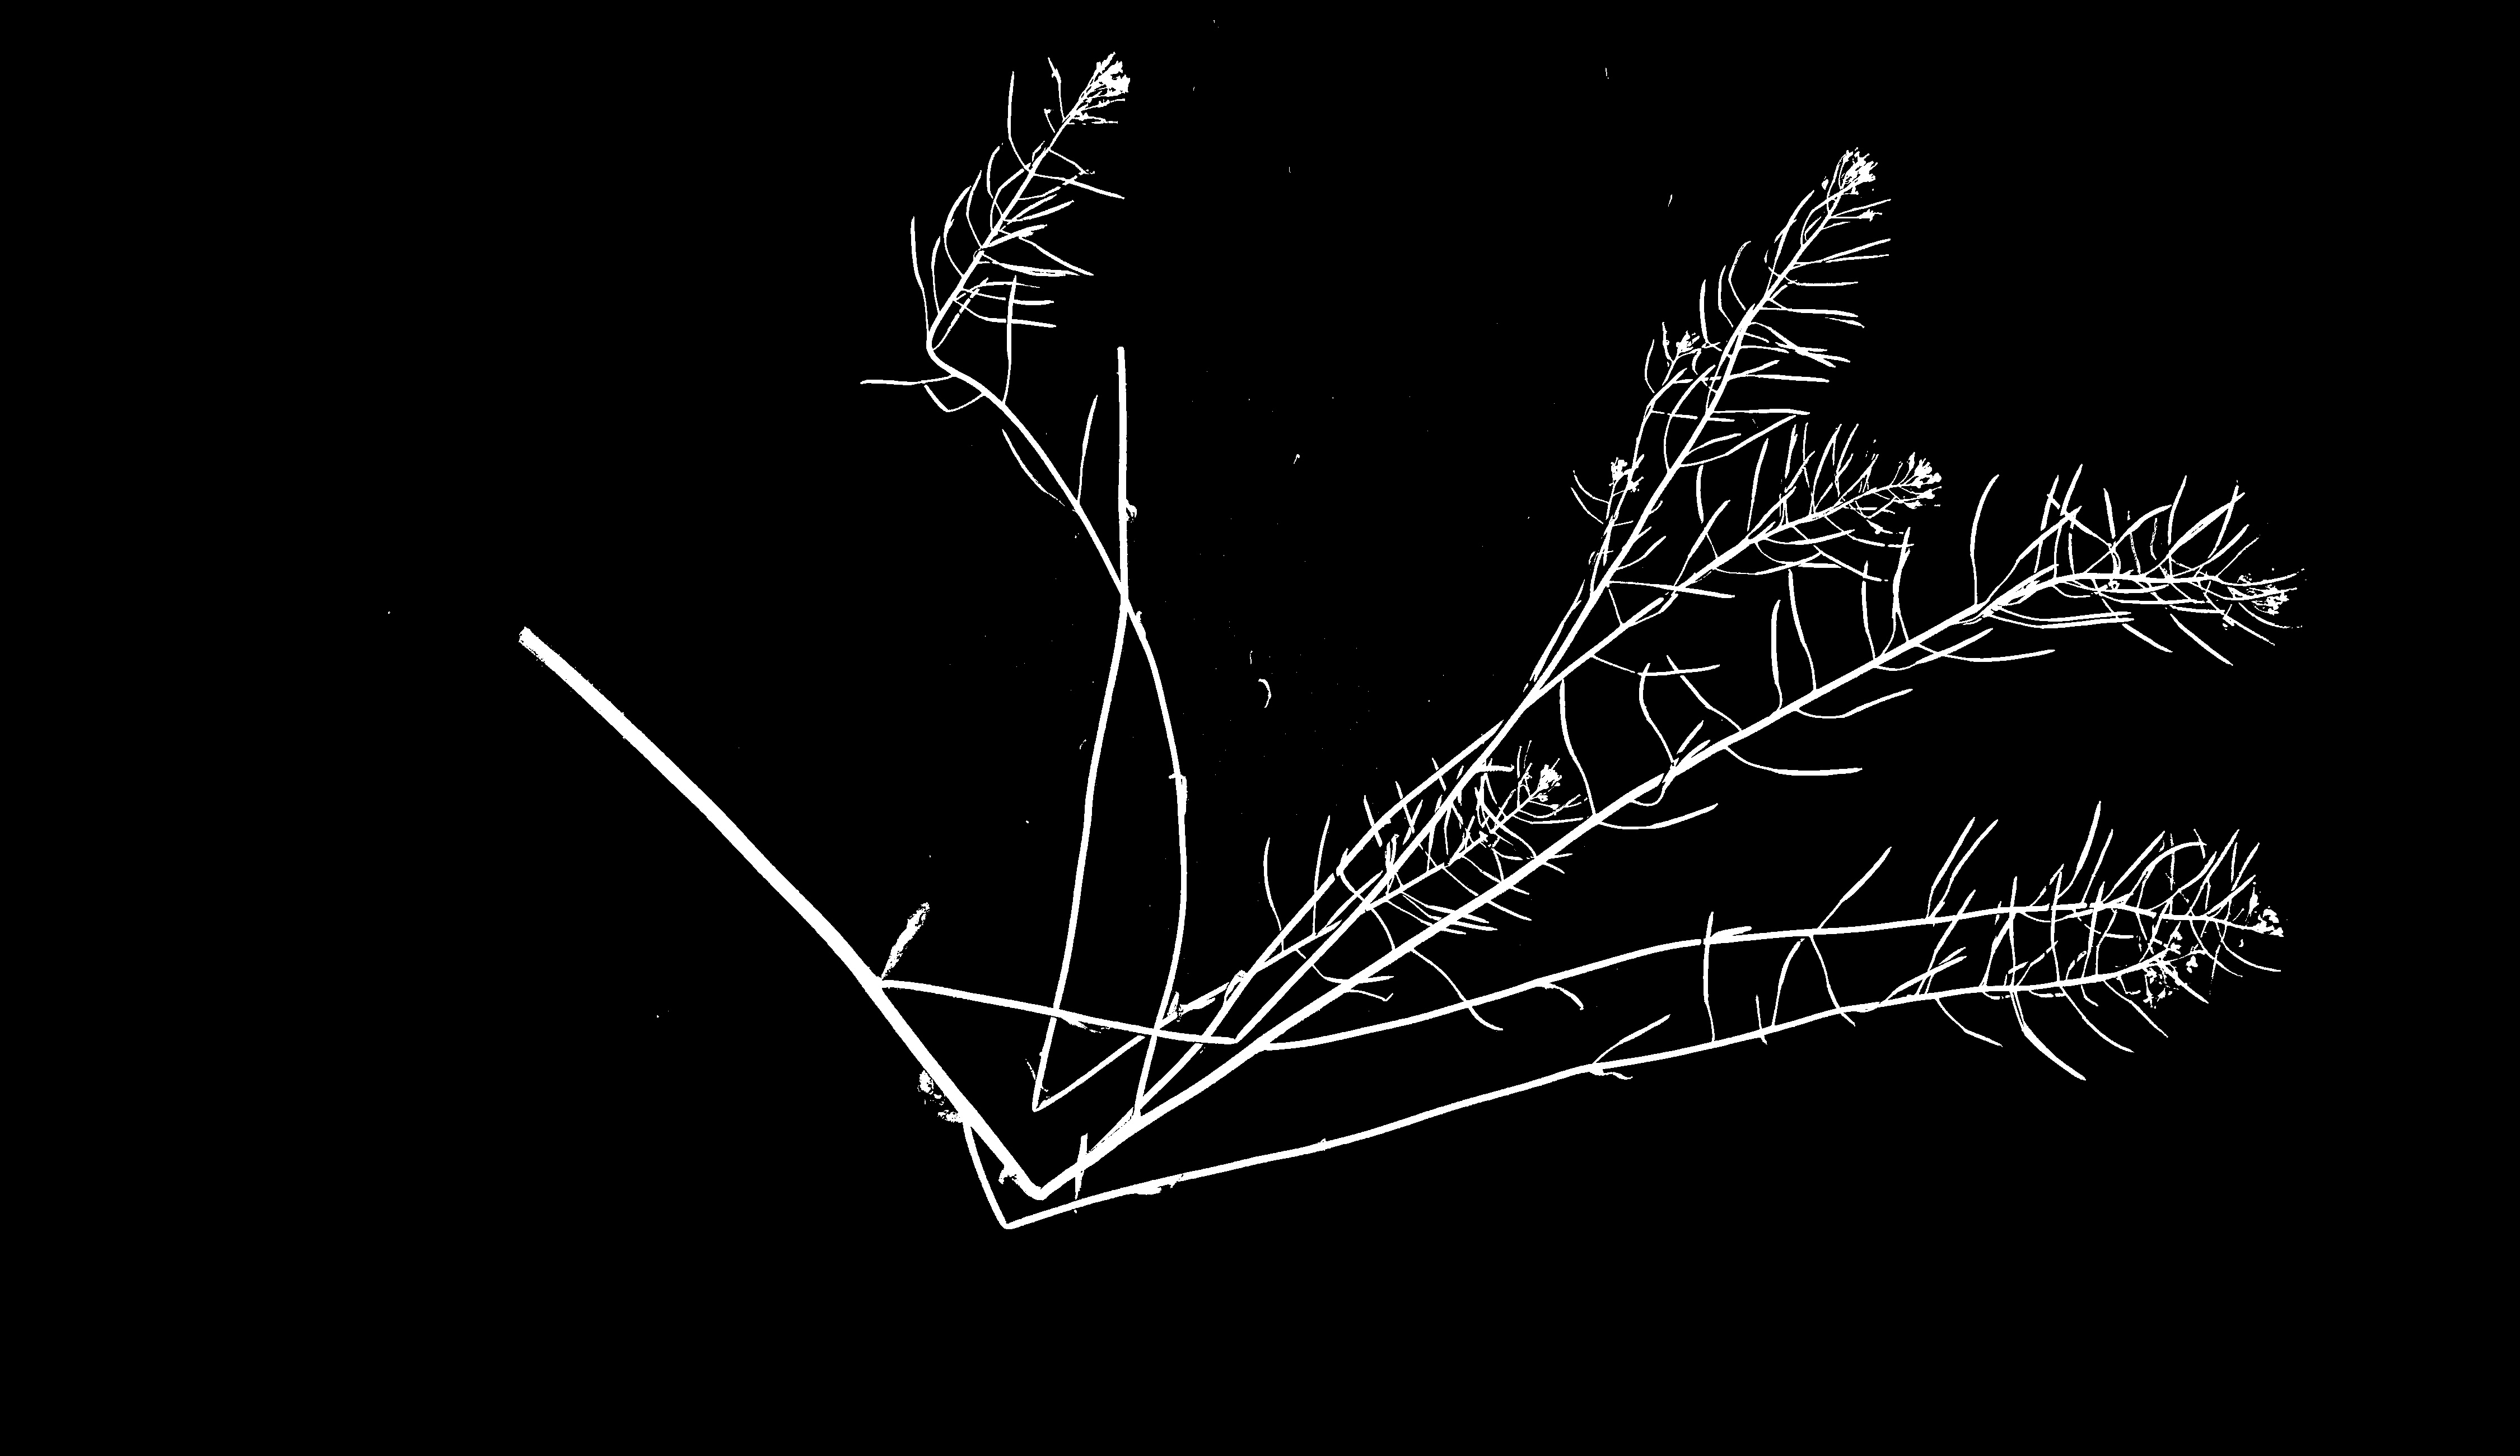
\includegraphics[width=\linewidth]{../figs/P1060902.JPG_proc.jpeg}
        \caption{} \label{fig:segmented}
    \end{subfigure}
    \begin{subfigure}[t]{0.45\textwidth}
        \centering
        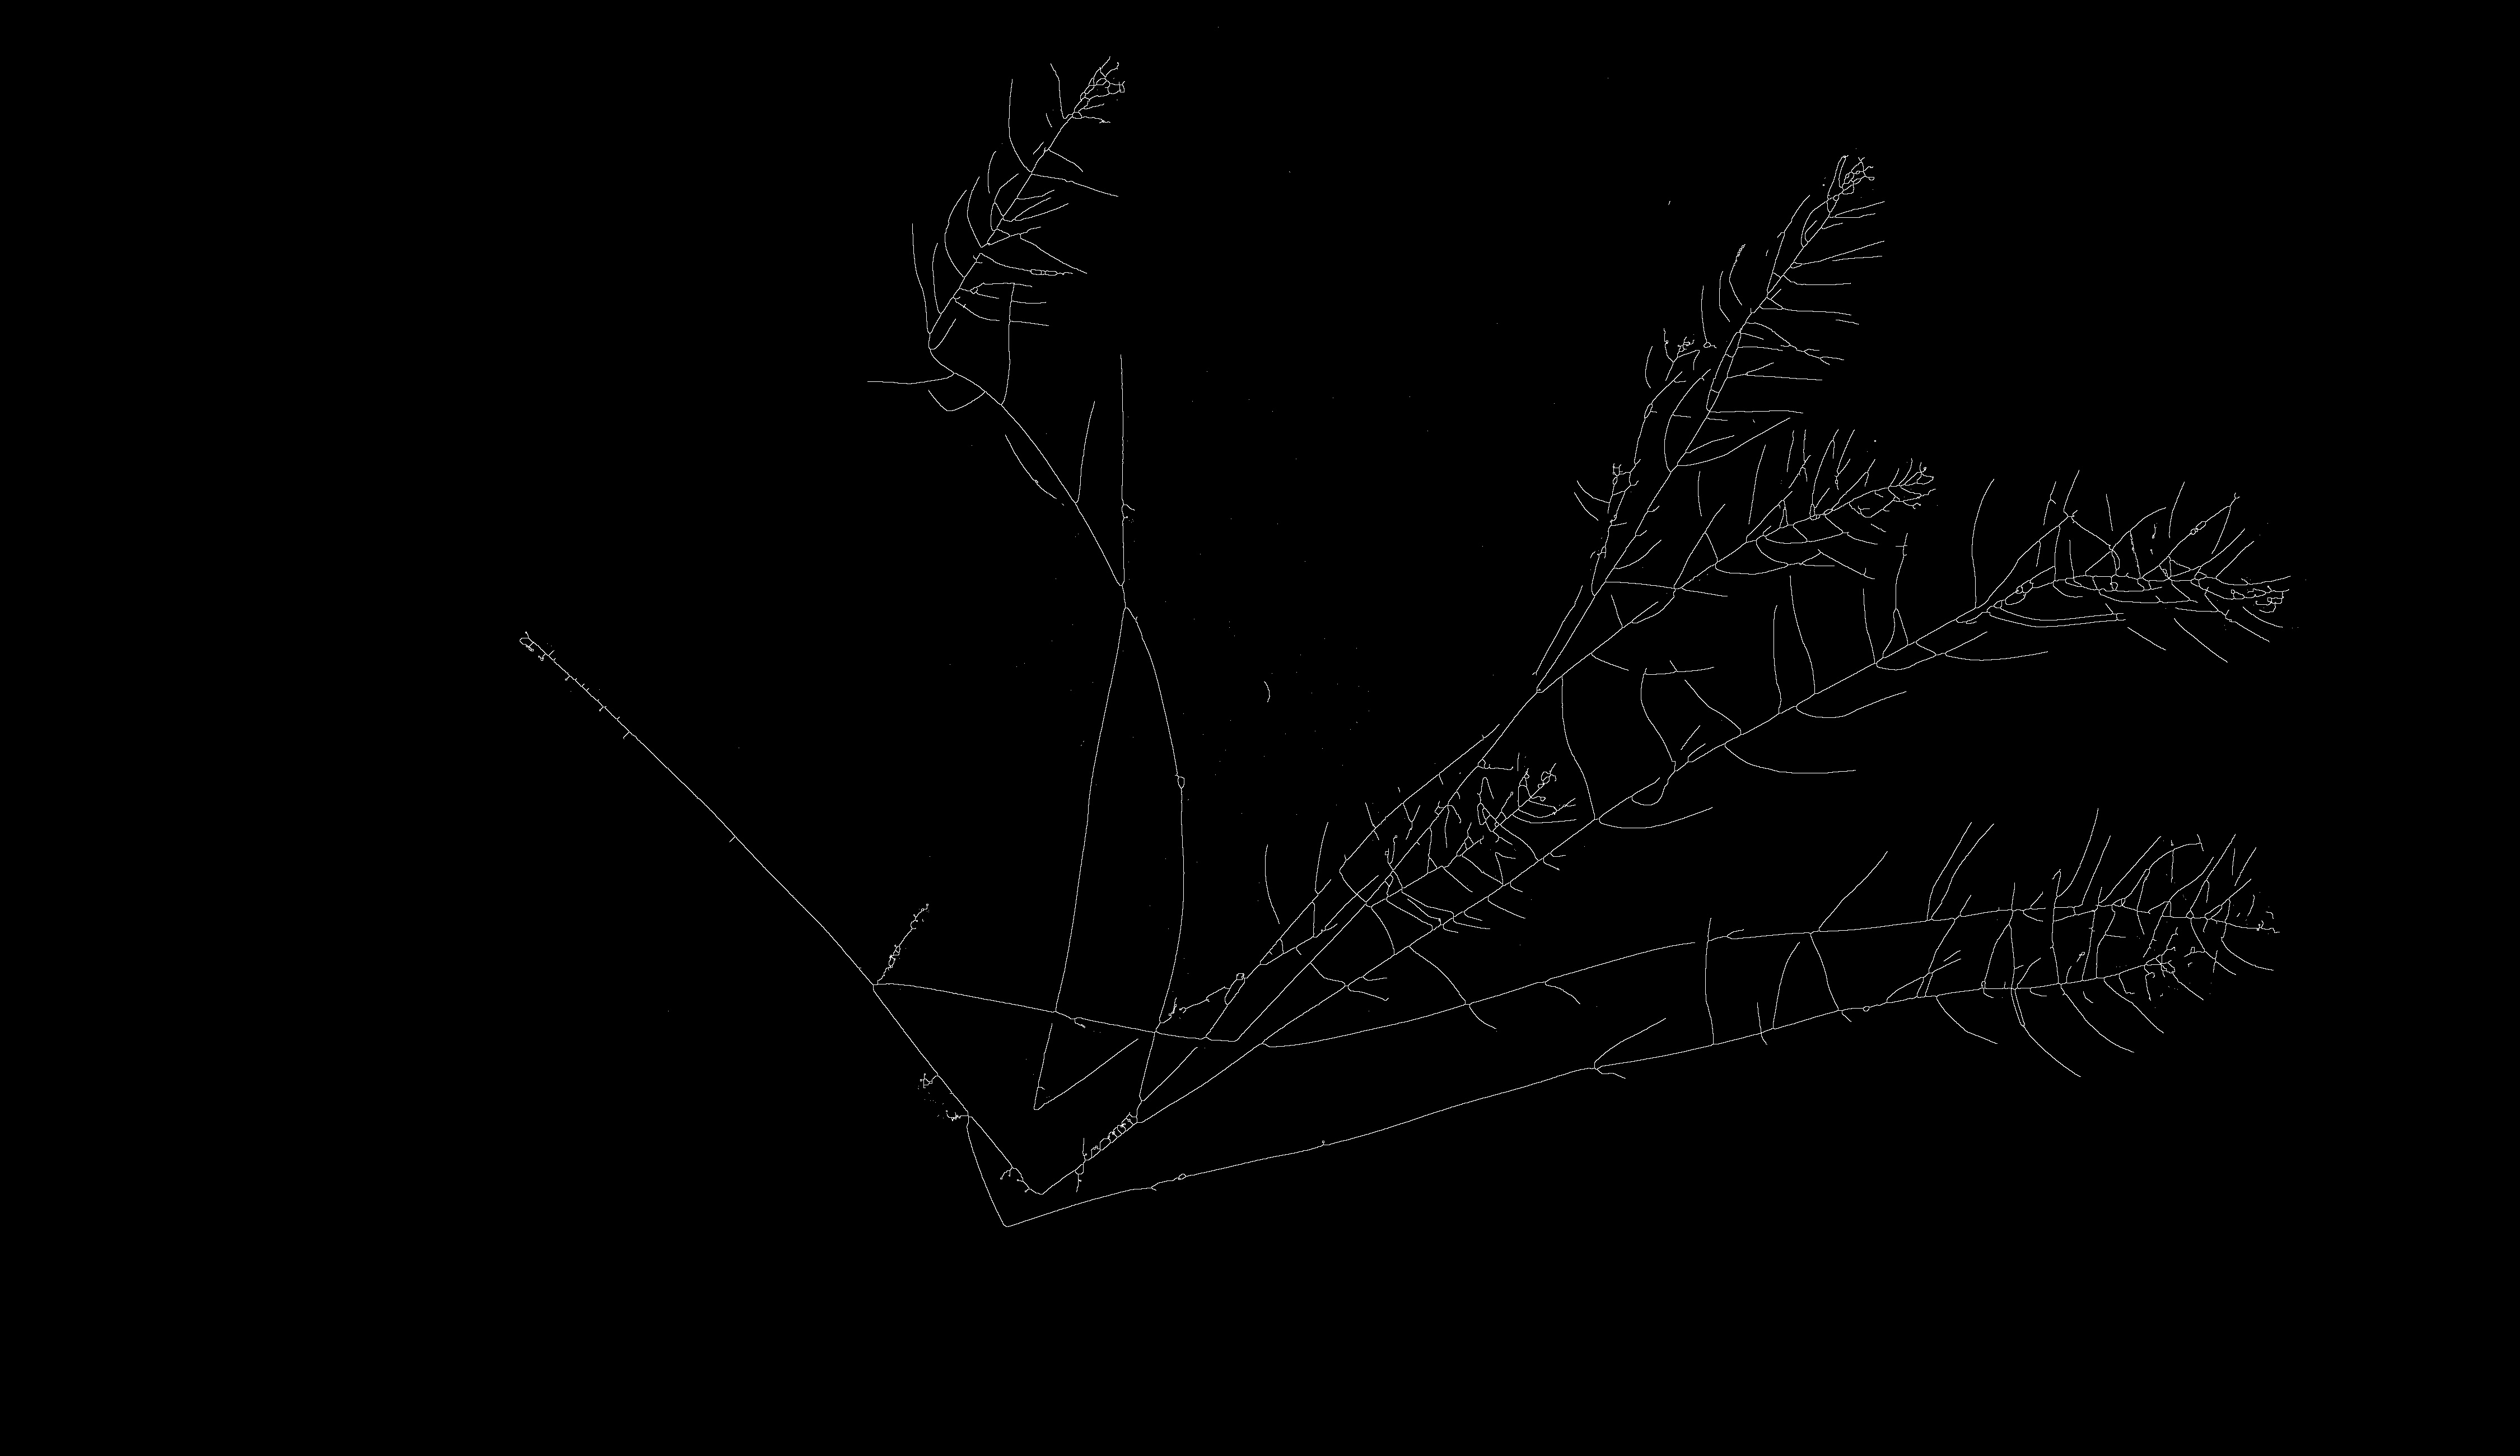
\includegraphics[width=\linewidth]{../figs/P1060902.JPG_proc_sk.jpeg}
        \caption{} \label{fig:sk}
    \end{subfigure}
        \begin{subfigure}[t]{0.45\textwidth}
        \centering
        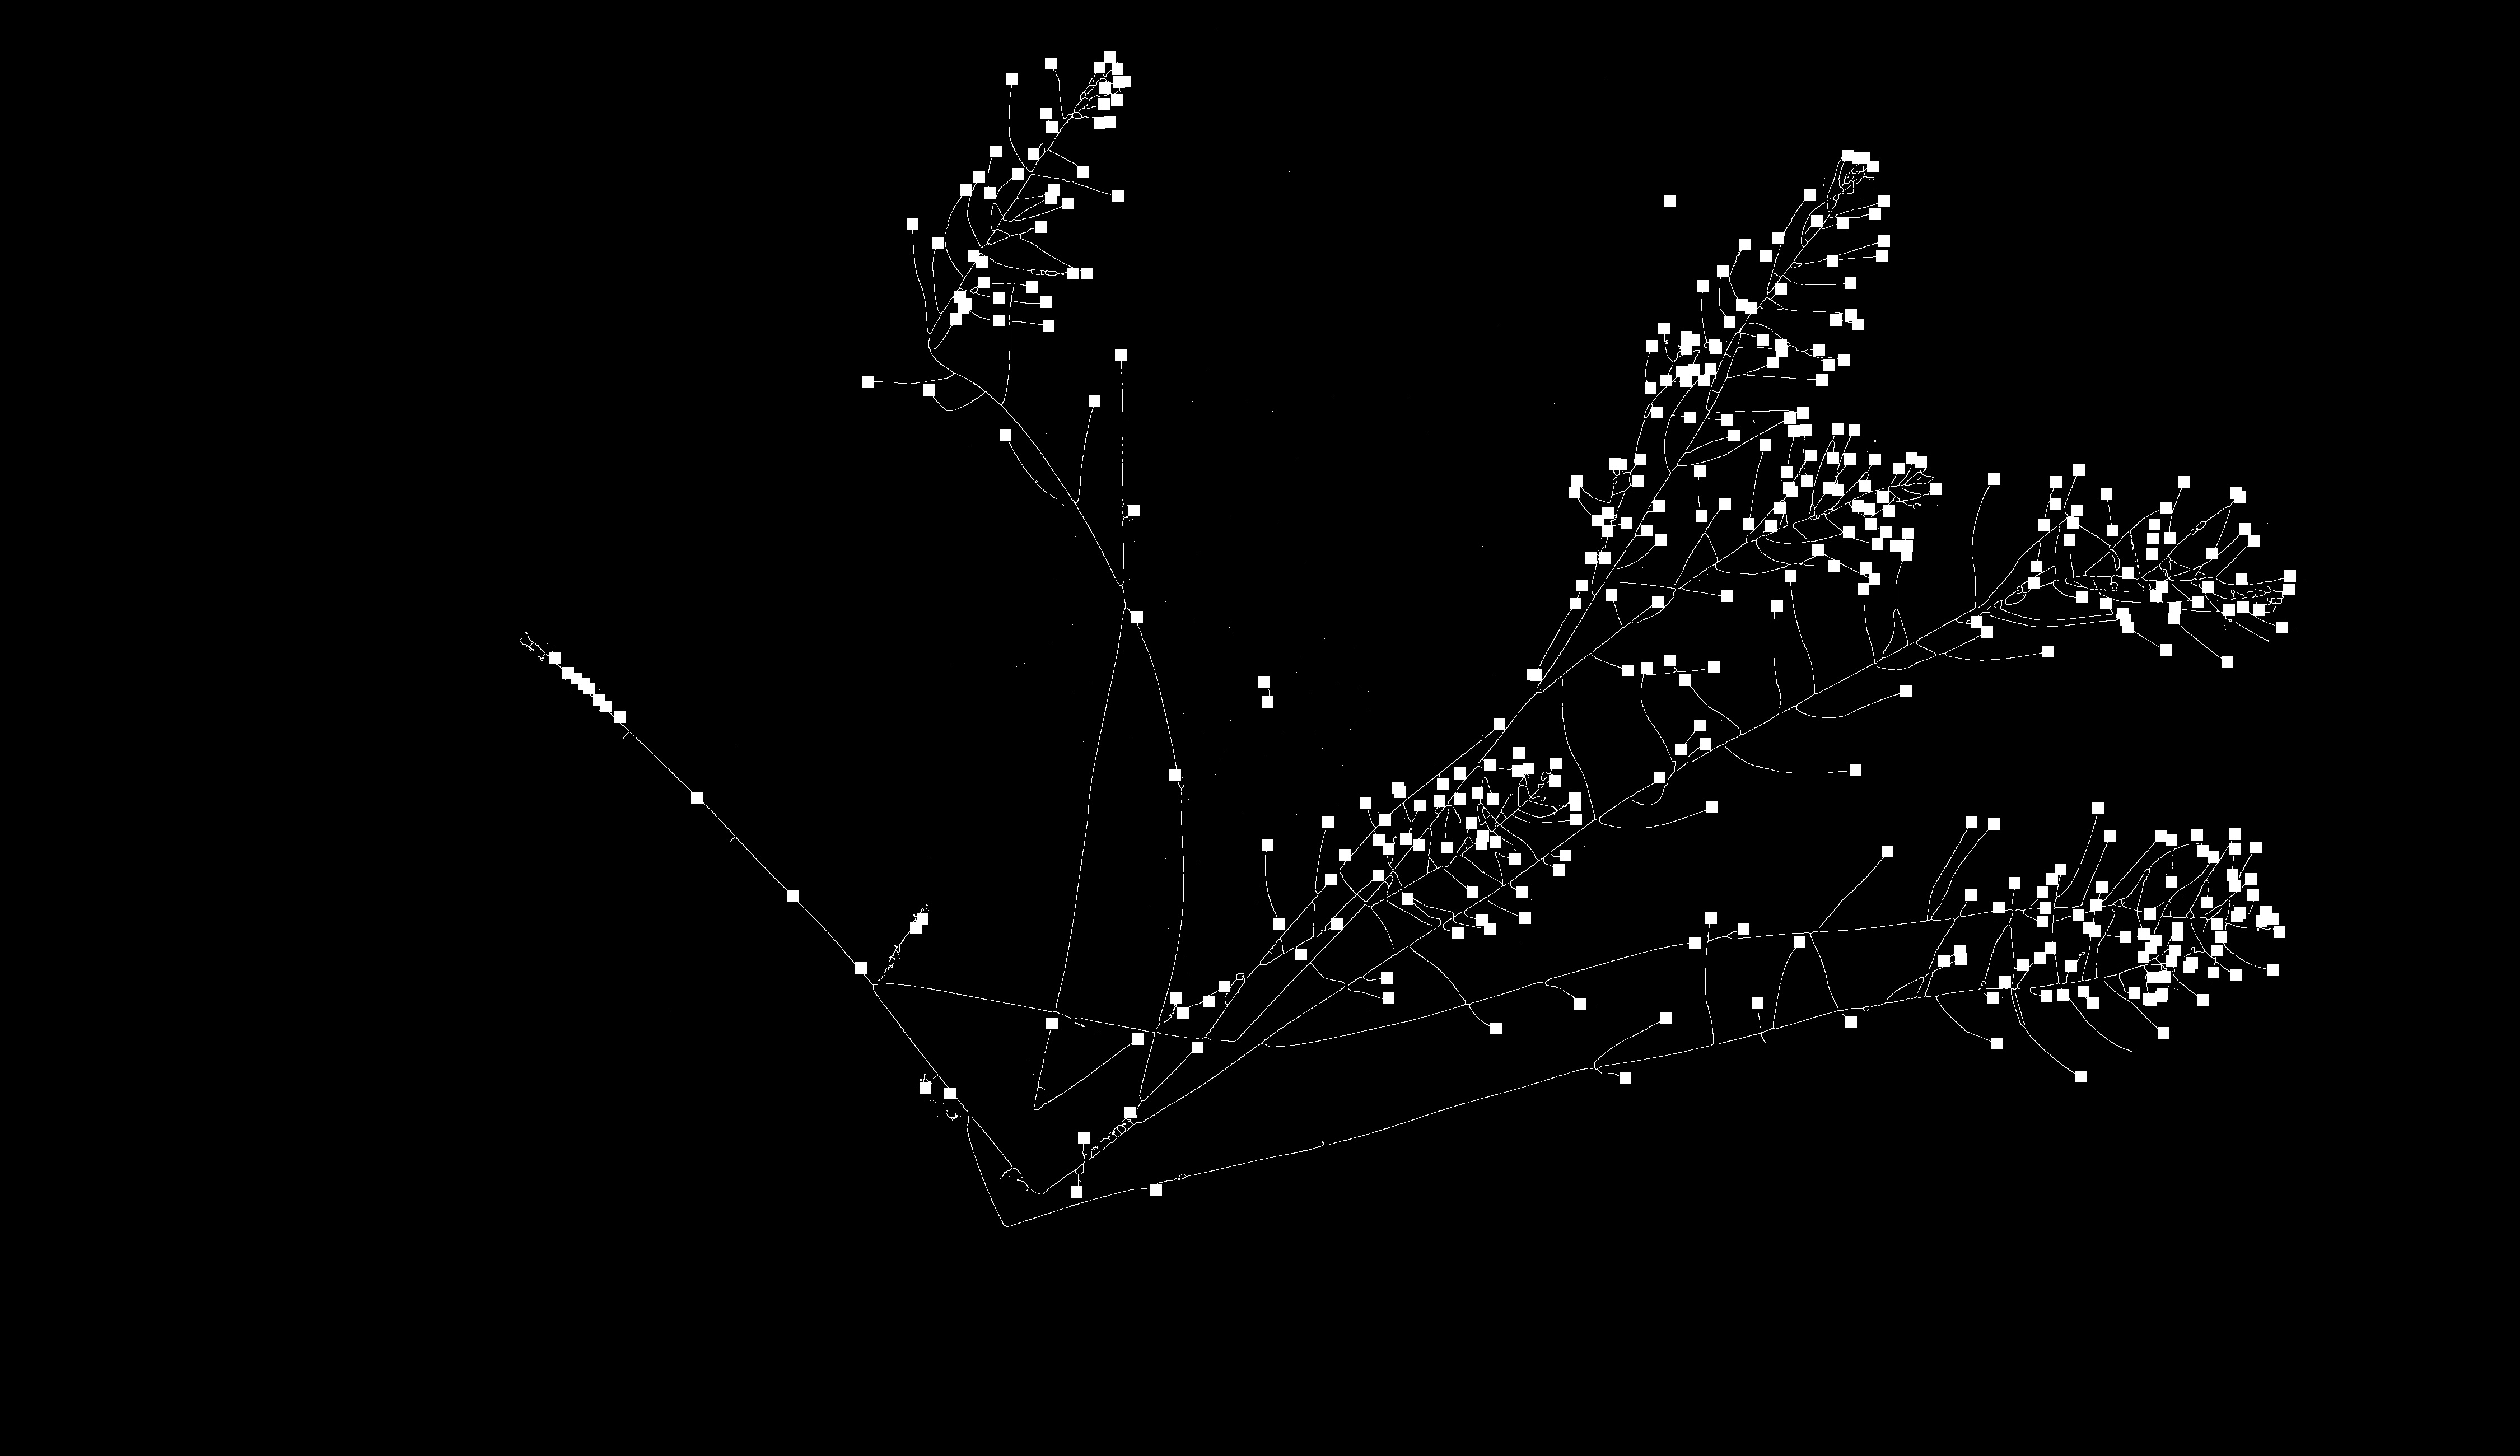
\includegraphics[width=\linewidth]{../figs/P1060902.JPG_proc_ends.jpeg}
        \caption{} \label{fig:ep}
    \end{subfigure}
    \begin{subfigure}[t]{0.45\textwidth}
        \centering
        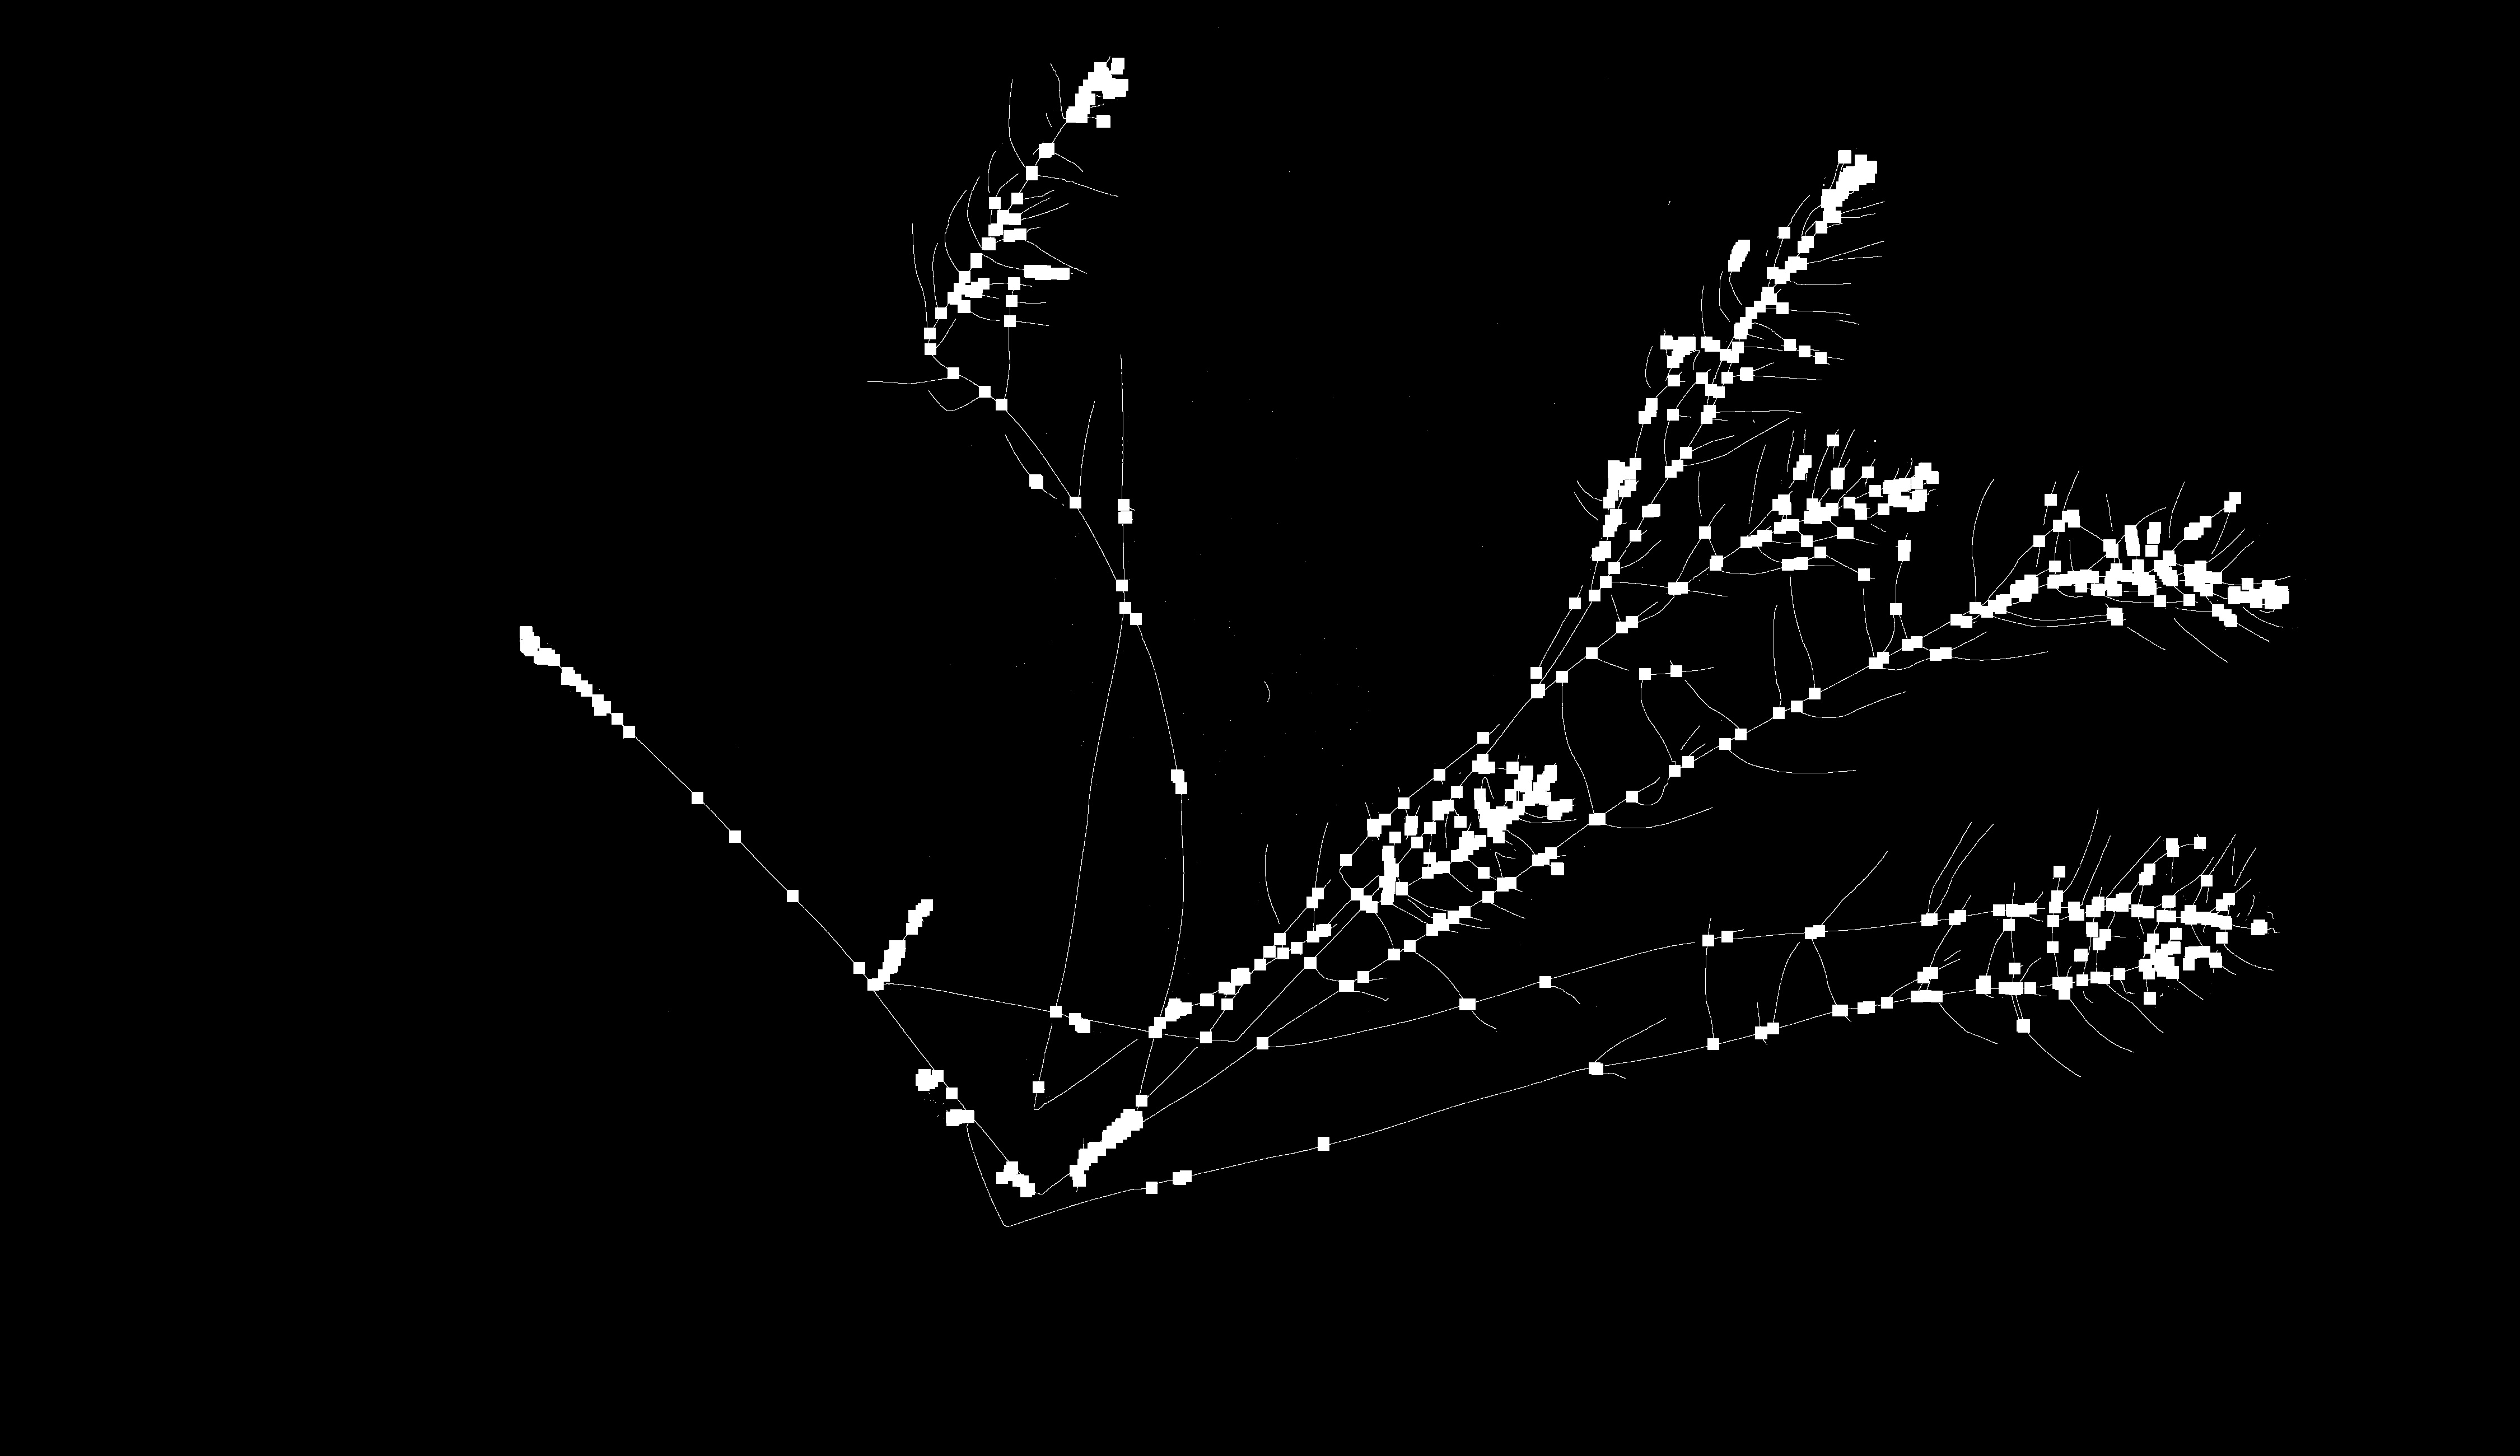
\includegraphics[width=\linewidth]{../figs/P1060902.JPG_proc_branches.jpeg}
        \caption{} \label{fig:bp}
    \end{subfigure}
\caption{Example sakeletonisation results from raw image (\subref{fig:original}) to segmented (\subref{fig:segmented}), skeletonised (\subref{fig:sk}), the detected branches (\subref{fig:bp}) and endpoints (\subref{fig:ep}).}
\label{fig:skeletonisation}
\end{figure}

\begin{figure}
    \centerline{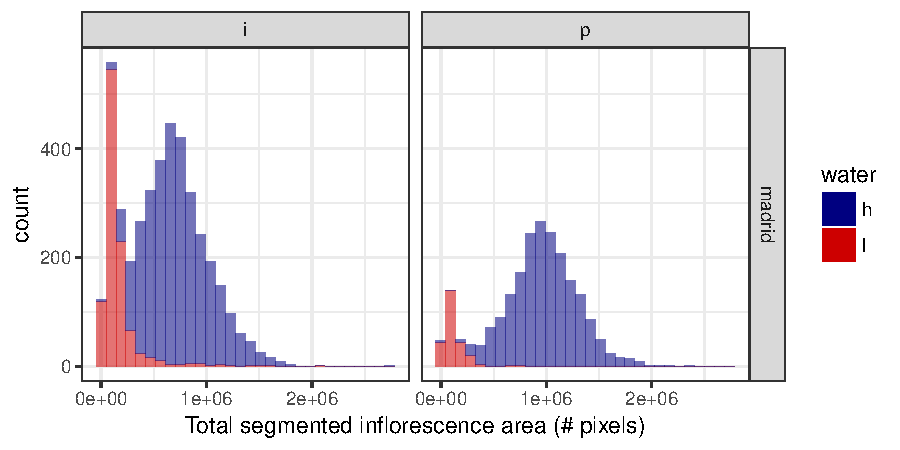
\includegraphics[width=5in]{../figs/Figure_inflorescence_distribution.pdf}}
    \caption{ Distribution of total inflorescence size (number of pixels)}
    \label{fig:inflorescence}
\end{figure}

\begin{figure}
    \centerline{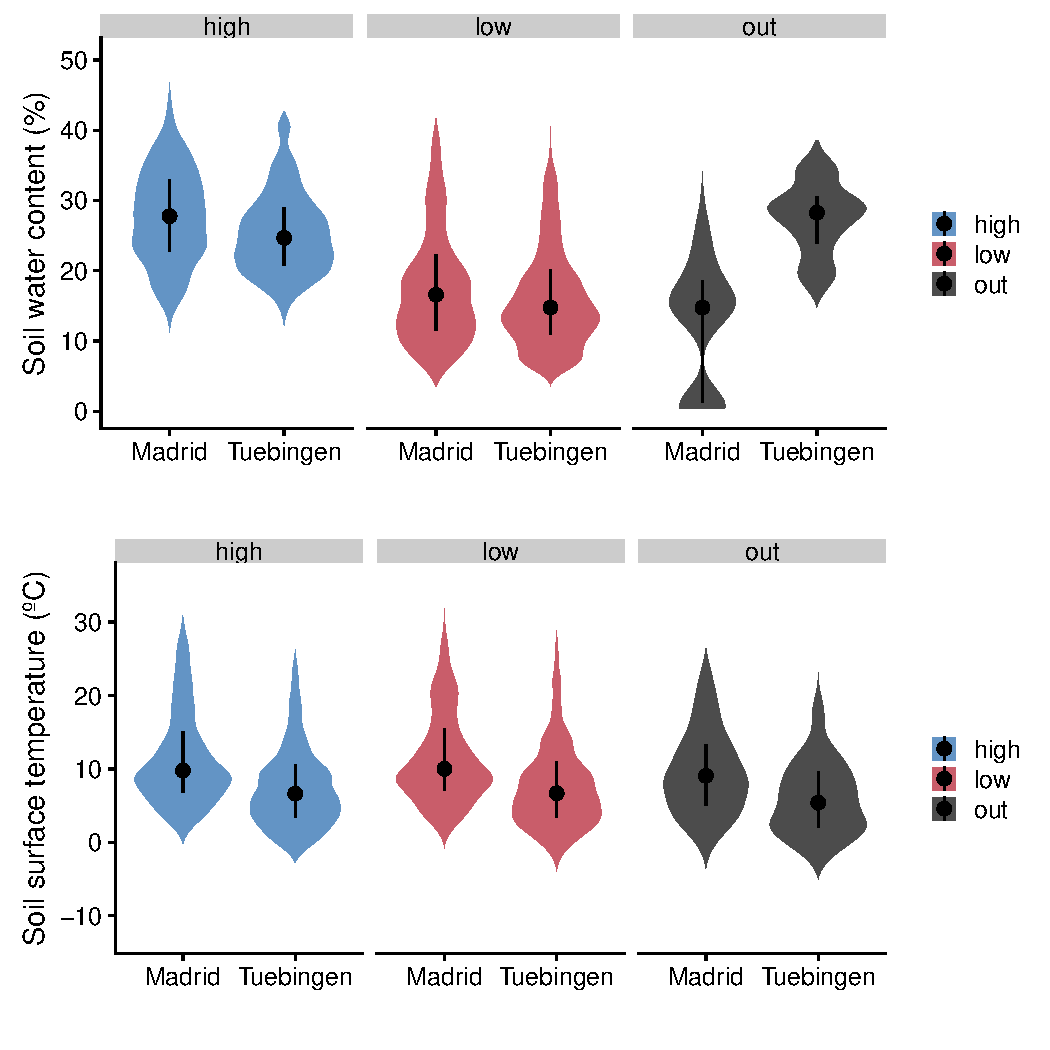
\includegraphics[width=5in]{../figs/Figure_watering_temperature.pdf}}
    \caption{ Soil water content and temperature from the 35 sensors monitororing each experimental block and the conditions outside the tunnel.}
    \label{fig:histoenv}
\end{figure}

\hypertarget{refs}{}
\hypertarget{ref-1001_Genomes_Consortium2016-nw}{}
1001 Genomes Consortium. (2016). 1,135 genomes reveal the global pattern
of polymorphism in arabidopsis thaliana. \emph{Cell}, \textbf{166},
481--491. Retrieved from
\url{http://dx.doi.org/10.1016/j.cell.2016.05.063}

\hypertarget{ref-Bates2015-ly}{}
Bates, D., Mächler, M., Bolker, B. \& Walker, S. (2015). Fitting linear
Mixed-Effects models using lme4. \emph{Journal of Statistical Software,
Articles}, \textbf{67}, 1--48. Retrieved from
\url{https://www.jstatsoft.org/v067/i01}

\hypertarget{ref-Bolker2009-by}{}
Bolker, B.M., Brooks, M.E., Clark, C.J., Geange, S.W., Poulsen, J.R.,
Stevens, M.H.H. \& White, J.-S.S. (2009). Generalized linear mixed
models: A practical guide for ecology and evolution. \emph{Trends Ecol.
Evol.}, \textbf{24}, 127--135. Retrieved from
\url{http://dx.doi.org/10.1016/j.tree.2008.10.008}

\hypertarget{ref-Exposito-Alonso2017-ob}{}
Exposito-Alonso, M., Vasseur, F., Ding, W., Wang, G., Burbano, H.A.A. \&
Weigel, D. (2017). Genomic basis and evolutionary potential for extreme
drought adaptation in arabidopsis thaliana. \emph{bioRxiv}, 118067.
Retrieved from \url{http://dx.doi.org/10.1101/118067}


\end{document}
